\def\chapname{Mathematical Model}
\chapter[\chapname]{
\chapname \chapsubhead{The results of this chapter are published in \cite{ABG2012modeling}.}}

\label{chap:math-model}

\begin{abstract}
In this chapter, we provide a mathematical model for the
electrolocation problem. We first investigate
the forward admittivity equation and derive the
approximate boundary conditions on the skin of the fish. Then we
provide a dipole approximation for small targets away from the
fish. Finally, numerical simulations are performed in order to 
illustrate these results.
\end{abstract}


\section{Introduction}

Mathematically speaking, the electrolocation process
is an inverse problem for the
electric field created by the fish. Indeed, given the current
distribution over the skin,  the problem is to recover the
conductivity distribution in the surrounding space. Hence, 
in order to lead a quantitative investigation of this process,
we have to model the electric field precisely. The aim of this chapter is to 
do so for the particular case of the electrolocation of an object around the fish.


Two problems arise: the direct problem, \emph{i.e.}, the equations
involved and their boundary conditions. 
Here, we will make precise the model of 
Assad~\cite{assad1997phd,assad1990hypercube}. As already mentioned in
section~\ref{sub:modelisation_champ_bio}, if
$u$ denotes the scalar potential field, it involves
the equation $\Delta u=0$ on the exterior of the body,
and Robin boundary conditions on the skin :
\begin{equation}
u-\xi\frac{\partial u}{\partial\nu}=\psi,\label{eq:assad_BC}
\end{equation}
 where $\psi$ is the potential inside the body and $\xi=h(\sigma_{0}/\sigma_{s})$
($h$ being the skin thickness and $\sigma_{s}$ (resp.
$\sigma_{0}$) the skin (resp. water) conductivity) is the
\emph{effective skin thickness}. 

The second problem is to image a target. In this perspective,
we generalize formula (\ref{eq:dipole_rasnow}) to the case of a
non-uniform background electric field, taking into account the
distortion induced by the body of the fish, and with any shape of
the target. This approximation will be then very useful in chapter~\ref{chap:localization} and,
in some way, re-interpreted in chapters~\ref{chap:GPT-extraction} and~\ref{chap:pnas}. 

This chapter is organized as follows. In section
\ref{sec:forward_problem}, the physical model is set up and the
equations governing the electric field are introduced and their
basic properties analyzed. Using layer potential techniques, the
boundary condition (\ref{eq:assad_BC}) is rigorously recovered in
section \ref{sub:BC-derivation}. In
subsection~\ref{sec:perturbation-target}, asymptotic expansions will
be carried out for the electric field in the presence of a small
and distant target.
Finally, numerical simulations of the electric field -~with or without
a target~- are performed in section
\ref{sec:numeric-direct}. Due to the presence of a hyper-singular
operator, a particular attention is paid to the numerical scheme
for solving the direct problem.

%Reconstructions of the electromagnetic parameters and the size of
%disk- and ellipse-shaped targets are also provided.


\section{Physical modeling}

\label{sec:forward_problem}

The aim of this section is to formulate the \emph{forward
problem}. The electromagnetic formulation is introduced in
subsection \ref{sub:setup}. The model equations are
non-dimensionalized in subsection \ref{nondimension} and the
different scales identified. Subsection \ref{problemsetup} is
devoted to the problem setup. Existence, uniqueness and a useful
representation formula for the solution of the model equations are
proved in subsection \ref{sub:existence-uniqueness}.


\subsection{Electromagnetic formulation}

\label{sub:setup}

In this subsection, we derive the equations governing the electric
field. A formal explanation of the electroquasistatic (or EQS)
formulation is given.

The electroquasistatic (or EQS) formulation is a low-frequency
limit for the Maxwell system in three dimensions~\cite{vanRienen2001}. In the frequency
domain, the latter is given by
\begin{equation}
\left\{ \begin{alignedat}{1}\nabla\cdot\varepsilon {E} & =\rho,\\
\nabla\cdot {B} & =0,\\
\nabla\times {E} & =-i\omega {B},\\
\nabla\times\frac{ {B}}{\mu} & = {j}+i\omega\varepsilon {E},
\end{alignedat}
\right.\label{eq:maxwell}
\end{equation}
where $E$ is the electric field, $B$ is the magnetic induction
field, $\rho$ and $j$ are the free charges and currents, $\omega$
is the frequency, $\mu$ is the magnetic permeability, and
$\varepsilon$ is the electric permittivity. Moreover, in a medium
of conductivity $\sigma$, Ohm's law connects the electric field to
the induced current density (${j_{i}}=\sigma {E}$) so the total
current density can be decomposed as:
\[
{j}=\sigma {E}+ {j_{s}},
\]
 where ${j_{s}}$ is a source of current (in our model, it
comes from the electric organ). Then, taking the divergence of the
last line in (\ref{eq:maxwell}), we have:
\begin{equation}
\nabla\cdot(\sigma+i\varepsilon\omega) {E}=-\nabla\cdot
{j_{s}}.\label{eq:div-maxwell4}
\end{equation}
The EQS approximation consists of considering the electric field
as irrotational because the magnetic field variation is
negligible. A sufficient condition for that is given by
\cite{vanRienen2001}:
\begin{equation}
\frac{L_{\textrm{max}}}{\lambda_{\textrm{min}}}\ll1,\label{eq:eqs_condition}
\end{equation}
 where $L_{\textrm{max}}$ is the maximal length of the problem and $\lambda_{\textrm{min}}$
the minimal wavelength. Here, we can take $L_{\textrm{max}}=1$m because
the range of electrolocation does not exceed two body lengths
\cite{moller1995electric}. In the water, the minimal wavelength is given
by
\[
\lambda_{\textrm{min}}=\frac{1}{\omega_{\textrm{max}}\sqrt{\mu\varepsilon}},
\]
 where $\mu\approx\mu_{0}$, $\varepsilon\approx80\varepsilon_{0}$
and $\omega_{\textrm{max}}$ is the maximal frequency emitted by the
fish, which is of the order of $10$kHz. Thus, the fraction in
(\ref{eq:eqs_condition}) is of order $10^{-4}$, so the EQS
approximation is very well suited for our situation.

Going back to the equation of the electric field
(\ref{eq:div-maxwell4}), we can now use the fact that ${E}$ is
irrotational to state that it is derived from a  scalar potential
field $u$. This finally leads us to the following equation:
\begin{equation}
\nabla\cdot(\sigma+i\varepsilon\omega)\nabla u=-\nabla\cdot
{j_{s}}.\label{eq:EQS-PDE}
\end{equation}


To conclude, taking into account the slow variation of the
electric field leads us to consider an admittivity equation (the \emph{admittivity} being
$\sigma + i \omega \varepsilon$) instead of a conductivity equation (\ie with $\sigma$ only).
However, for the rest of this section, the
imaginary part of this admittivity will be neglected; indeed
measurements on a \emph{Gnathonemus petersii} showed that the
capacitance (\ie $\omega \varepsilon$\footnote{It is also called \emph{susceptance} when it does
not come from capacitive effects only, as it is the case here.}) of the skin, the body, and the water are
very small compared to their respective
conductivity~\cite{caputi1998electric,scheich1973coding}. Thus,
this EQS approximation will be used only in the presence of a
target: it will be detected by the phase shift induced by its
capacitance.


\subsection{Non-dimensionalization} \label{nondimension}
In this subsection, the setup of the problem is
non-dimensionalized. The first step consists in identifying the
different scales of the model problem. The electric potential $u$,
the variables $x$ and $\omega$, and the parameters $\sigma$ and
${j_{s}}$ can be written as follows:
\[
u=V_{0}u',\;
x=Lx',\;\omega=\omega_{0}\omega',\;\sigma=\sigma_{0}k,\;
{j_{s}}=\frac{I_{0}}{L^{2}} {j_{s}'},
\]
 where $V_{0}$ is the voltage produced by an \emph{electric organ
discharge} (EOD), $L$ is the length of the fish, $\omega_{0}$ is
the fundamental frequency of the EOD, $\sigma_{0}$ is the
conductivity of the surrounding water and $I_{0}$ is the current
intensity inside the electric organ. Moreover, anticipating the
next subsection, the conductivity of the body and the skin play an
important role in the shape of the electric field. Thus, in the
list of parameters we add the conductivity of the body
$\sigma_{b}$, the thickness of the skin $\delta_s$ and its surface
conductivity $\Sigma$. The orders of magnitude of these parameters
are found in Table~\ref{tab:Orders-of-magnitude}.

\begin{table}[!h]
\centering%
\begin{tabular}{|c|c|c|}
\hline
Quantity  & Order of magnitude  & Reference\tabularnewline
\hline
\hline
$V_{0}$  & $10$ mV  & \cite{assad1998electric,stoddard1999electric}\tabularnewline
\hline
$L$  & $10$ cm  & \cite{moller1995electric}\tabularnewline
\hline
$\omega_{0}$  & $1$ kHz  & \cite{moller1995electric}\tabularnewline
\hline
$\sigma_{0}$  & $100$ $\mu$S$\cdot$cm$^{-1}$  & \cite{maciver2001prey}\tabularnewline
\hline
$I_{0}$  & $1$ mA  & \cite{bell1976electric}\tabularnewline
\hline
$\sigma_{b}$  & $1$ S$\cdot$m$^{-1}$  & \cite{scheich1973coding}\tabularnewline
\hline
$\Sigma$  & $100$ $\mu$S$\cdot$cm$^{-2}$  & \cite{caputi1998electric}\tabularnewline
\hline
$\delta_s$  & $100$ $\mu$m  & \cite{zakon1986electroreceptive}\tabularnewline
\hline
\end{tabular}

\caption{\label{tab:Orders-of-magnitude}Orders of magnitude of the
physical quantities involved. These are only scales and not the
exact values measured in the cited references. Here $S$ is Siemens
($1S =1A/1V$).}
\end{table}


These $n=8$ quantities involve $r=4$ fundamental units of the SI
system, so according to the Buckingham-Pi theorem, we need $n-r=4$
nondimensional quantities to describe the model problem. The first
one can be found by rewriting the equation (\ref{eq:EQS-PDE}) in
terms of the nondimensional quantities ($x^\prime, k, u',
j_{s}^\prime$):
\begin{equation}
\nabla_{x'}\cdot
k\nabla_{x'}u'=-\frac{I_{0}}{\sigma_{0}V_{0}L}\nabla\cdot
{j_{s}'}.\label{eq:nondimensionalized-EQS}
\end{equation}
% Note that the order of magnitude for the conductivity used here is
%$\sigma_{b}$ because the electric organ is located inside the body
%(in most species, it is found in the tail~\cite{moller1995electric}).

The multiplicative term in the right-hand side of the previous
equation is not important as the equation is linear. The three
other nondimensional quantities come from the parameters of the
skin and the body of the fish:
\[
k_{b}:=\frac{\sigma_{b}}{\sigma_{0}}\sim10^{2},\; k_{s}:=\frac{h\Sigma}{\sigma_{0}}\sim10^{-2},\;h:=\frac{\delta_s}{L}\sim10^{-3}.
\]
 In other words, in nondimensional units, $k_{b}$ (resp. $k_{s}$)
is the body (resp. skin) conductivity and $h$ is the skin thickness.

To conclude, omitting the prime symbol for the sake of clarity and
denoting by $k_b J_s$ the source term in equation
(\ref{eq:nondimensionalized-EQS}), the governing PDE is the
following
\begin{equation}
\nabla\cdot k\nabla u= k_b J_s,\label{eq:EQS-final}
\end{equation}
 where $k$ is piecewise constant, being equal to $1$ in the water,
$k_{b}$ inside the body of the fish and $k_{s}$ in the skin. These
domains will be specified in the next subsection.

For the sake of simplicity, from now on, we only consider  the
model equations in two dimensions.

\subsection{Problem setup} \label{problemsetup}

The setup is as follows: the body occupies a fixed smooth open set
$\Omega_{b}$ and the skin with constant thickness is denoted by
$\Omega_{s}$.
 The source of the electric field is a sum of Dirac functions:
\begin{equation} \label{sumdirac}
J_s= \sum_{j=1}^{m}\alpha_{j}\delta_{x_s^{(j)}},
\end{equation}
 where, for $1\leq j\leq m$, $x_s^{(j)}\in\Omega_{b}$ and $J_s$ satisfies
 the charge neutrality condition
\begin{equation} \label{neutre}
\ds \sum_{j=1}^m \alpha_{j}=0.
\end{equation}
Although condition (\ref{neutre}) is the physical condition in our
model, we will show how to modify the derivations and the results
of the paper in the general case. An illustration is given in
Figure~\ref{fig:Setup}.
\begin{figure}
\centering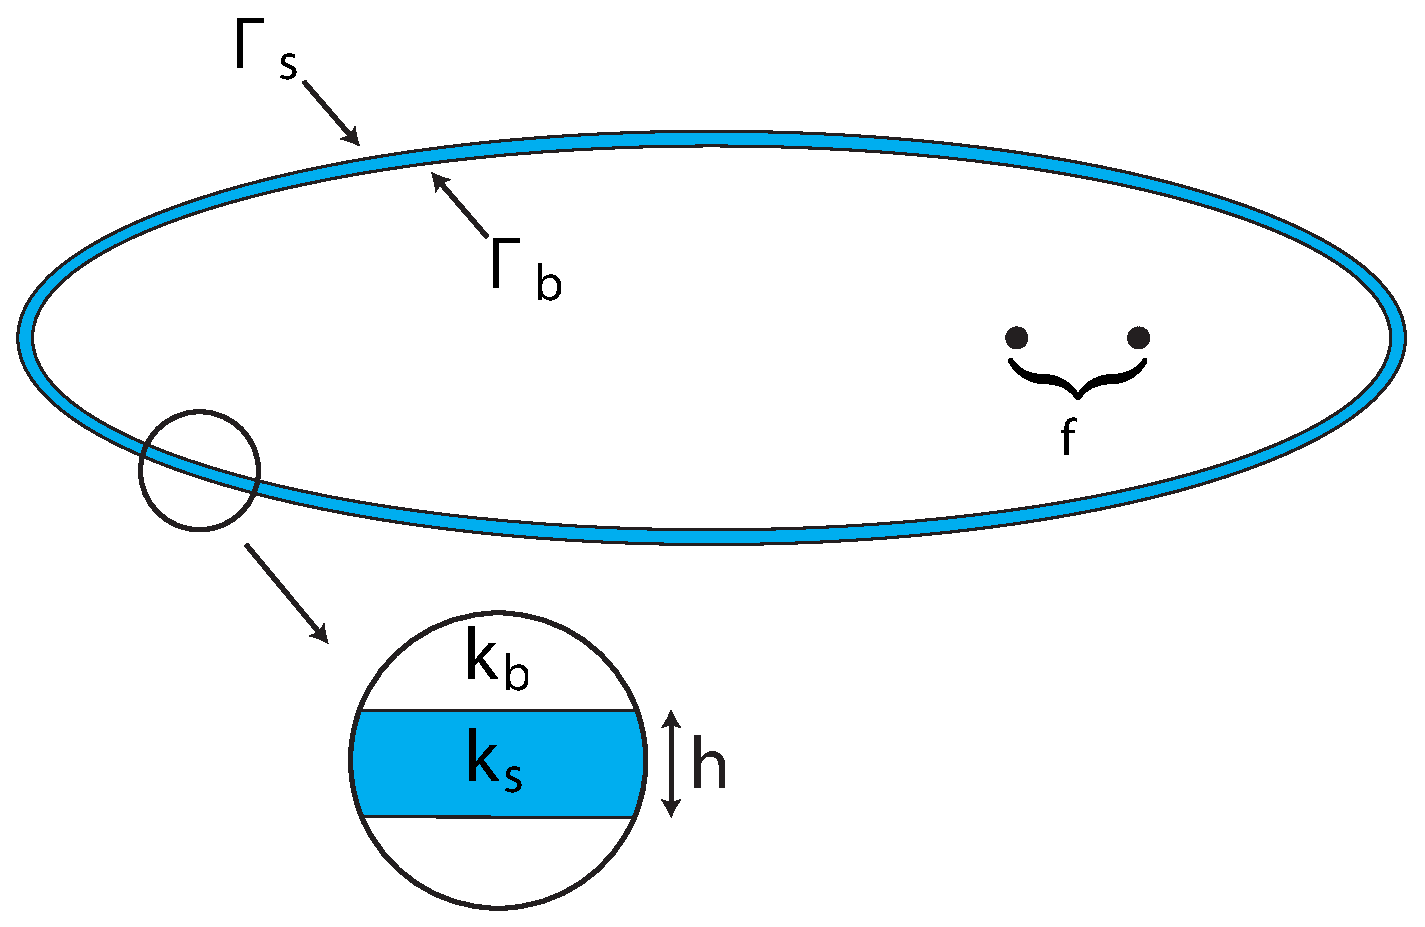
\includegraphics[width=10cm]{model/fish_model.eps}
\caption{Setup of the problem. The conductivities are
non-dimensionalized so that $\sigma_{0}=1$. The body $\Omega_{b}$,
with boundary $\Gamma_b$ and conductivity $k_b$, is the interior
of the ellipse. The skin $\Omega_{s}$, with exterior boundary
$\Gamma_s$ and conductivity $k_s$, is represented in blue. The
sources $J_s$ are given by the two dots. \label{fig:Setup}}
\end{figure}

Our main purpose is to investigate the behavior of the solution of
(\ref{eq:EQS-final}) with
\begin{equation} \label{defk}
k(x)=\left\{\begin{array}{l} k_s \quad \mbox{if } x \in \Omega_s,\\
\nm k_b \quad \mbox{if } x \in \Omega_b,\\
\nm 1 \quad \mbox{otherwise},
\end{array}
\right.
\end{equation}
where $k_s \neq 1$ and $k_b \neq k_s$. Let $\xi$ be the effective
thickness given by \cite{assad1990hypercube}:
\begin{equation} \label{defxi}
\xi:=\frac{h}{k_{s}}.
\end{equation}

In order to make the dependence of the solution on $h$ and
$k_b$ clear ($\xi$ being fixed), let us denote such a solution by
$u_{h,k_{b}}$. Adding a far field condition (essential for
uniqueness, see subsection \ref{sub:existence-uniqueness}), it is
the solution of
\begin{equation}
\left\{ \begin{alignedat}{2}\nabla\cdot k\nabla u_{h,k_{b}} & = k_b J_s, & \,\, x\in\mathbb{R}^{2},\\
\left|u_{h,k_{b}} \right| & = {O}(\left|x\right|^{-1}), &
\,\,\left|x\right|\rightarrow\infty \text{ uniformly in }\hat{x},
\end{alignedat}
\right.\label{eq:governing_equation}
\end{equation}
 where $\hat{x}:=x/\left|x\right|$ and $k(x)$ is given by
 (\ref{defk}).

 In the next subsection, we analyze
equation~(\ref{eq:governing_equation}) and show that there exists
a unique solution that can be represented as the sum of a harmonic
function and two single-layer potentials.

\subsection{Existence, uniqueness, and representation of the
electric potential} \label{sub:existence-uniqueness}

We first prove  the uniqueness of the solutions
of~(\ref{eq:governing_equation}) and then we derive a
representation formula, which will give us the existence of the
solution. For the moment, $h$ and $k_{b}$ are fixed, but we
suppose that:
\begin{equation}
k_{s} < 1 < k_{b}.\label{eq:ordering_conductivities}
\end{equation}



\subsubsection{Uniqueness}

The uniqueness comes from the second line
of~(\ref{eq:governing_equation}) \cite{ammari2007polarization}.
Indeed, let $v=u_1-u_2$, where $u_1$ and $u_2$ are two solutions
of (\ref{eq:governing_equation}) and let us show that $v=0$.
From~(\ref{eq:ordering_conductivities}) we get, for $R$
sufficiently large (so that the ball with center $0$ and radius
$R$ encompasses $\Omega_s$):
\begin{align*}
\int_{\left|x\right|<R}\left|\nabla v\right|^{2}
\leq\frac{1}{k_{s}} \int_{\left|x\right|<R} k(x) \left|\nabla
v\right|^{2} =
 \frac{1}{k_{s}}\int_{\left|x\right|=R}v\frac{\partial v}{\partial\nu}=
 -\frac{1}{k_{s}}\int_{\left|x\right|>R}\left|\nabla
v\right|^{2}\leq0.
\end{align*}
Here we have used the fact that  $\nabla v \in
L^2(\mathbb{R}^{2}\setminus \overline{\Omega}_s)$, which holds as
a consequence of the far field condition.
 A unique continuation argument shows that
$\left|\nabla v\right|^{2}=0$ in $\mathbb{R}^{2}$ and thus $v$ is
constant. Then, using the fact that $v\rightarrow0$ as
$|x|\rightarrow \infty$, we have $v=0$.


\subsubsection{Existence and representation}

The existence is given by a representation formula decomposing the
solution into a source part and a refraction part. This refraction
part implies layer potentials on the boundaries of the body and
the skin. Let us define them explicitly and give some well-known
results. First, let us introduce the following boundaries:
\[
\Gamma_{b}:=\partial\Omega_{b}\mbox{ and
}\Gamma_{s}:=\partial\Omega_{s}\setminus\Gamma_{b},
\]
and assume that they are of class $\mathcal{C}^{1,\eta}$ for some
$\eta >0$. In the following, the index $\beta$ stands for the
subscript $b$ or $s$. The single- and double-layer potentials on
$\Gamma_{\beta}$ are operators that map any $\varphi\in
L^{2}(\Gamma_{\beta})$ to $\mathcal{S}_{\beta} \varphi$ and
$\mathcal{D}_{\beta} \varphi$, respectively, where
\begin{equation}
\begin{aligned}\begin{aligned}\mathcal{S}_{\beta} := \mathcal{S}_{\Gamma_\beta} \mbox{ with } &
 (\mathcal{S}_\Gamma \varphi)(x):=\int_{\Gamma}G(x-s)\varphi(s)ds,\\
\mathcal{D}_{\beta} := \mathcal{D}_{\Gamma_\beta} \mbox{ with }  &
(\mathcal{D}_{\Gamma}\varphi)(x)
 :=\int_{\Gamma}\frac{\partial
G}{\partial\nu_{s}}(x-s)\varphi(s)ds,
\end{aligned}
\end{aligned}
\label{eq:def_single_layer}
\end{equation}
 where $G$ is the fundamental solution of the Laplacian in
 $\mathbb{R}^{2}$:
 \begin{equation} \label{defG}
 G(x) := \frac{1}{2\pi} \ln |x|, \quad x \neq 0.
 \end{equation}
For $\varphi\in L^{2}(\Gamma_{\beta})$, the functions
$\mathcal{S}_{\beta}\varphi$ and $\mathcal{D}_{\beta}\varphi$ are
harmonic functions in $\mathbb{R}^{2}\setminus\Gamma_{\beta}$;
their singularities hold on $\Gamma_{\beta}$. To describe these
singularities, we define, for a function $w$ defined in
$\mathbb{R}^{2}\setminus\Gamma_{\beta}$ and $x\in\Gamma_{\beta}$:
\[
\begin{aligned}\left.w(x)\right|_{\pm} & :=\lim_{t\rightarrow0}w(x\pm t\nu(x)),\\
\left.\frac{\partial w}{\partial\nu}(x)\right|_{\pm} & :=\lim_{t\rightarrow0}
 \nabla w(x\pm t\nu(x)) \cdot \nu(x) .
\end{aligned}
\]
 Across the boundary~$\Gamma_{\beta}$, the following  trace relations
hold~\cite{ammari2007polarization}:
\begin{equation}
\begin{aligned}\left.\mathcal{S}_{\beta}\varphi\right|_{+} & =\left.\mathcal{S}_{\beta}\varphi\right|_{-},\\
\left.\frac{\partial\mathcal{S}_{\beta}\varphi}{\partial\nu}\right|_{\pm} & =\left(\pm\frac{1}{2}I+\mathcal{K}_{\beta}^{*}\right)\varphi,\\
\left.\mathcal{D}_{\beta}\varphi\right|_{\pm} & =\left(\mp\frac{1}{2}I+\mathcal{K}_{\beta}\right)\varphi,\\
\left.\frac{\partial\mathcal{D}_{\beta}\varphi}{\partial\nu}\right|_{+} & =\left.\frac{\partial\mathcal{D}_{\beta}\varphi}{\partial\nu}\right|_{-}.
\end{aligned}
\label{eq:jump_formulas}
\end{equation}
 Here, for a $\mathcal{C}^{1,\eta}$-boundary $\Gamma_{\beta}$, the operator $\mathcal{K}_{\beta}$ and its $L^{2}$-adjoint
$\mathcal{K}_{\beta}^{*}$ are given by
\begin{equation}
\begin{aligned}\begin{aligned}\mathcal{K}_{\beta} := \mathcal{K}_{\Gamma_\beta} \mbox{ with } & 
(\mathcal{K}_{\Gamma_\beta}\varphi)(x)  :=\frac{1}{2\pi}\int_{\Gamma_{\beta}}\frac{
\langle (s-x) , \nu(s) \rangle}{\left|x-s\right|^{2}}\varphi(s)ds & ,\,\, x\in\Gamma_{\beta},\\
\mathcal{K}_{\beta}^* := \mathcal{K}_{\Gamma_\beta}^* \mbox{ with } & 
(\mathcal{K}_{\Gamma_\beta}^{*}\varphi)(x)  :=\frac{1}{2\pi }
\int_{\Gamma_{\beta}}\frac{ \langle (s-x) , \nu(x) \rangle
}{\left|x-s\right|^{2}}\varphi(s)ds & ,\,\, x\in\Gamma_{\beta},
\end{aligned}
\end{aligned}
\label{eq:def_Neumann_Poincare}
\end{equation}
where $\langle , \rangle$ denotes the scalar product in $\R^2$.
 From (\ref{eq:jump_formulas}) it
follows that the following jump formulas hold:
$$
\left.\frac{\partial\mathcal{S}_{\beta}\varphi}{\partial\nu}\right|_{+}
-
\left.\frac{\partial\mathcal{S}_{\beta}\varphi}{\partial\nu}\right|_{-}
= \varphi \quad \mbox{and} \quad
\left.\mathcal{D}_{\beta}\varphi\right|_{+} -
\left.\mathcal{D}_{\beta}\varphi\right|_{-} = - \varphi.
$$
The following invertibility result is useful
\cite{escauriaza1992,kellogg2010foundations,verchota1984}.
\begin{theorem} \label{theorem:invertibility_lambda_K}Suppose that
$\Gamma_{\beta}$ is $\mathcal{C}^{1,\eta}$ for some $\eta >0$.
Then the operator $\lambda I-\mathcal{K}_{\beta}^{*}$ is
invertible on $L_{0}^{2}(\Gamma_{\beta}):=\{ \varphi \in
L^2(\Gamma_{\beta}) : \int_{\Gamma_\beta} \varphi =0\}$ if
$\left|\lambda\right|\geq1/2$, and for $\lambda\in ( -\infty, -
1/2]\cup (1/2,+\infty)$, $\lambda I-\mathcal{K}_{\beta}^{*}$ is
invertible on $L^{2}(\Gamma_{\beta})$.
\end{theorem} 
Let us remark here that, when $\partial \Omega$ is connected, it is admitted
to use the simplified notations $\mathcal{S}_{\Omega}$, $\mathcal{D}_{\Omega}$ and
$\mathcal{K}_{\Omega}$~\cite{ammarikang2009}.

With these essentials tools, we can now prove the following
decomposition formula in the same spirit as in \cite{kang1996}:
\begin{lemma} \label{lemlatter} The solution of
problem~(\ref{eq:governing_equation}), with $J_s$ given by
(\ref{sumdirac}), can be written as
\begin{equation}
u(x)=p_s(x)+(\mathcal{S}_{s}\tilde{\varphi_{s}})(x)+(\mathcal{S}_{b}\varphi_{b})(x),\label{eq:decomposition_formula}
\end{equation}
 where
\begin{equation}
p_s(x)=\sum_{j=1}^{m}\alpha_{j}G(x-x_s^{(j)}),\label{eq:definition_H}
\end{equation}
 and the pair $(\tilde{\varphi_{s}},\varphi_{b})\in L^{2}(\Gamma_{s})\times L^{2}(\Gamma_{b})$
is uniquely determined by the system
\begin{equation}
\left\{ \begin{alignedat}{2}(\lambda_{s}I-\mathcal{K}_{s}^{*})\tilde{\varphi_{s}}-\frac{\partial\mathcal{S}_{b}\varphi_{b}}{\partial\nu} & =\frac{\partial p_s}{\partial\nu}, & \,\, x\in\Gamma_{s},\\
(\lambda_{b}I - \mathcal{K}_{b}^{*})\varphi_{b} -
\frac{\partial\mathcal{S}_{s}\tilde{\varphi_{s}}}{\partial\nu} & =
\frac{\partial p_s}{\partial\nu}, & \,\, x\in\Gamma_{b}.
\end{alignedat}
\right.\label{eq:definition_phis_phib}
\end{equation}
Here, $\lambda_b$ and $\lambda_s$ are given by
\begin{equation} \label{deflambdas}
\lambda_{s}:=\frac{k_{s}+1}{2(k_{s}-1)}\mbox{ and
}\lambda_{b}:=\frac{k_{s}+k_{b}}{2(k_{s}-k_{b})}.
\end{equation}
Moreover, the decomposition (\ref{eq:decomposition_formula}) of
$u$ into a source part $p_s$ and a refraction part
$\mathcal{S}_{s}\tilde{\varphi_{s}}+\mathcal{S}_{b}\varphi_{b}$ is
unique.\end{lemma}

\proof The system~(\ref{eq:governing_equation}) is equivalent to
the following transmission problem~\cite{allaire2007numerical}:
\begin{equation} \label{eqs210}
\left\{ \begin{alignedat}{2}\Delta u & ={J_s}, & \,\, x\in\mathbb{R}^{2}\setminus(\Gamma_{b}\cup\Gamma_{s}),\\
\left.u\right|_{+}-\left.u\right|_{-} & =0, & \,\, x\in\Gamma_{b}\cup\Gamma_{s},\\
k_{s}\left.\frac{\partial u}{\partial\nu}\right|_{+}-k_{b}\left.\frac{\partial u}{\partial\nu}\right|_{-} & =0,
& \,\, x\in\Gamma_{b},\\
\left.\frac{\partial u}{\partial\nu}\right|_{+}-k_{s}\left.\frac{\partial u}{\partial\nu}\right|_{-} & =0, &
\,\, x\in\Gamma_{s},\\
\left|u\right| & = {O}(\left|x\right|^{-1}), &
\,\,\left|x\right|\rightarrow\infty,\text{ uniformly in }\hat{x}.
\end{alignedat}
\right.
\end{equation}
The existence of a solution $(\tilde{\varphi}_s, \varphi_b)$ to
(\ref{eq:definition_phis_phib}) comes from the fact that
$|\lambda_s|, |\lambda_b|  \in (1/2, + \infty)$  and Theorem
\ref{theorem:invertibility_lambda_K}. On the other hand, the functions
$\mathcal{S}_{s}\tilde{\varphi_{s}}$ and
$\mathcal{S}_{b}\varphi_{b}$ are harmonic in $\Omega_{b}$, and
according to the definition of $p_s$, we have $\Delta u= {J_s}$ in
$\Omega_{b}$. In $\Omega_{s}$ and
$\mathbb{R}^{2}\setminus\overline{\Omega}_{s}\cup
\overline{\Omega}_{b}$, all these functions are harmonic so we
have $\Delta u=0$. The trace relations on $\Gamma_b$ and
$\Gamma_s$ are then given by the singularities
(\ref{eq:jump_formulas}) of $\mathcal{S}_{s}$ and
$\mathcal{S}_{b}$ (see~\cite{ammari2007polarization}) since $p_s$ is
smooth away from the points~$x_s^{(j)}$. Finally, all these functions
are controlled by~$\left|x\right|^{-1}$
when~$\left|x\right|\rightarrow\infty$. In this way, the existence
of a solution to~(\ref{eq:governing_equation}) is proved.

To prove the uniqueness of the decomposition, let us take
$\tilde{\varphi_{s}}'$ and $\varphi_{b}'$ such that
\[
p_s+\mathcal{S}_{s}\tilde{\varphi_{s}}+\mathcal{S}_{b}\varphi_{b}=p_s+\mathcal{S}_{s}\tilde{\varphi_{s}}'+\mathcal{S}_{b}\varphi_{b}'.
\]
 Because of the location of the singularities, the function $\mathcal{S}_{s}(\tilde{\varphi_{s}}-\tilde{\varphi_{s}}')
 =\mathcal{S}_{b}(\varphi_{b}'-\varphi_{b})$
is harmonic in $\Omega_{s}\cup\overline{\Omega}_{b}$, which gives
by the jump formula for the normal derivative of $\mathcal{S}_{b}$
on $\Gamma_b$ that $\varphi_{b}=\varphi_{b}'$. Finally, applying
the jump formula for the normal derivative of $\mathcal{S}_{s}$ on
$\Gamma_s$, we have $\tilde{\varphi_{s}}=\tilde{\varphi_{s}}'$.
\cqfd





\section{Thin resistive skin and highly conductive body asymptotic}

\label{sub:BC-derivation}


In this section,  we derive the appropriate boundary conditions
associated with the presence of a very thin and very resistive
skin. Robin boundary conditions will be found after an asymptotic
analysis of the layer potentials involved.

We assume that $\Omega_{s}$ is described as:
\[
\Omega_{s}:=\big\{ x +t\nu(x),\,
x\in\partial\Omega_{b},\,0<t<h\big\},
\]
 where $\nu$ is the outward normal unit vector and consider the following asymptotic regime:
\begin{equation} \label{assumpk}
k_s = \frac{h}{\xi}, \quad \xi \mbox{ is fixed}, \quad
h\rightarrow0, \mbox{ and }k_{b}\rightarrow\infty \quad
(\mbox{so } k_s \rightarrow 0),
\end{equation}
where $\xi$ is the effective thickness. We compute the first-order
asymptotic $u_{0,\infty}$ of $u_{h,k_b}$ as $h
\rightarrow 0$ and $k_b\rightarrow +\infty$ and see that it is the
solution of the following system:
\begin{equation}
\left\{ \begin{alignedat}{2}\Delta u_{0,\infty} & ={J_s}, & \,\, x\in\Omega_{b},\\
\Delta u_{0,\infty} & =0, & \,\, x\in\mathbb{R}^{2}\setminus\overline{\Omega}_{b},\\
\left.u_{0,\infty}\right|_{+}-\left.u_{0,\infty}\right|_{-} & =\xi\left.\frac{\partial u_{0,\infty}}{\partial\nu}\right|_{+}, & \,\, x\in\partial\Omega_{b},\\
\left.\frac{\partial u_{0,\infty}}{\partial\nu}\right|_{-} & =0, & \,\, x\in \partial \Omega_{b},\\
\left|u_{0,\infty}\right| & = {O}(\left|x\right|^{-1}), &
\,\,\left|x\right|\rightarrow\infty,\text{ uniformly in }\hat{x}.
\end{alignedat}
\right.\label{eq:asymptotic_equation}
\end{equation}
Here, the subscripts $+$ and $-$ represent the limit from outside
and inside $\Omega_b$, respectively.  Note that in the limiting
model (\ref{eq:asymptotic_equation}), the role of $J_s$ is to fix
the potential $ u_{0,\infty} \big|_{-}$ on $\partial \Omega_{b}$.

For the system~(\ref{eq:asymptotic_equation}), Lemma
\ref{lemlatter} yields the following result.
\begin{lemma} \label{lemma:decomposition_lemma_asymptotic} Assume that (\ref{neutre}) holds. The solution
of problem~(\ref{eq:asymptotic_equation}) can be written as
\begin{equation}
u(x)=p_s(x)-\frac{1}{\xi}(\mathcal{S}_{b}\varphi)(x)+(\mathcal{D}_{b}\varphi)(x),
\label{eq:decomposition_formula_asymptotic}
\end{equation}
 where $\xi$ is defined by (\ref{defxi}), $p_s$ is given by (\ref{eq:definition_H}), and $\varphi\in L_0^{2}(\Gamma_{b}):= \{\phi \in L^2(\Gamma_b): \int_{\Gamma_b}
 \phi =0\}$
is given by the following integral equation:
\begin{equation} \label{eq:decomposition_formula_asymptotic2}
\frac{1}{\xi}\left(\frac{1}{2}I-\mathcal{K}_{b}^{*}\right)\varphi
+\frac{\partial\mathcal{D}_{b}\varphi}{\partial\nu}=-\frac{\partial
p_s}{\partial\nu}, \quad x \in \Gamma_b.
\end{equation}
 The decomposition (\ref{eq:decomposition_formula_asymptotic}) of $u$ into a source part and a refraction part is unique.
\end{lemma}
The proof of this lemma involves exactly the same arguments as in
the previous one: jump formulas applied to the operators.

The decomposition formulas~(\ref{eq:decomposition_formula}) and
(\ref{eq:decomposition_formula_asymptotic}) will be essential in
the next part to derive an asymptotic expansion of
$u_{h,k_{b}}$ as $h\rightarrow 0$ and $k_b\rightarrow
\infty$. To be more precise, we prove the following theorem:
\begin{theorem} \label{theorem:main-result}There exists a constant $C$
independent of $h$ and $k_{b}$ such that the following
inequality holds for $h$ and $1/k_{b}$ small enough:
\begin{equation}
\left\Vert u_{h,k_{b}}-u_{0,\infty}\right\Vert
_{L^{\infty}(\mathbb{R}^{2})}\leq
C\left(h+\frac{1}{k_{b}}\right),\label{eq:estimate-general}
\end{equation}
 where $u_{h,k_{b}}$ and $u_{0,\infty}$ are the solutions of (\ref{eq:governing_equation})
and (\ref{eq:asymptotic_equation}), respectively.
\end{theorem}


For doing so, we will perform asymptotic analysis of the layer
potentials introduced in the representation formula
(\ref{eq:decomposition_formula_asymptotic}) as $h \rightarrow
0$ and $k_b\rightarrow +\infty$ and show that the limiting
function is the solution of~(\ref{eq:asymptotic_equation}). We
will adapt the work done by Zribi in his thesis~\cite{zribilayer}
and by Zribi and Khelifi in \cite{khelifizribi2011asymptotic}. We will use the
decomposition formula for $u_{h,k_{b}}$ and compute
asymptotic expansions of the refraction part. The limiting
solution will then be $u_{0,\infty}$. This latter is well defined
if the limits $h\rightarrow0$ and $k_{b}\rightarrow\infty$
are independent, so we must seek the two following limits:
\[
\lim_{k_{b}\rightarrow\infty}\lim_{h\rightarrow0}u_{h,k_{b}}\mbox{ and }\lim_{h\rightarrow0}\lim_{k_{b}\rightarrow\infty}u_{h,k_{b}},
\]
 and show that they are the same. Zribi \cite[chapter 3]{zribilayer}
studied the case when $k_{b}$ remains fixed, with non-uniform
thickness of the skin $\Omega_{s}$; the limit $u_{0,1}$ is the
solution of the system:
\begin{equation}
\left\{ \begin{alignedat}{2}\Delta u_{0,1} & ={J_s}, & \,\, x\in\Omega_{b},\\
\Delta u_{0,1} & =0, & \,\, x\in\mathbb{R}^{2}\setminus\overline{\Omega}_{b},\\
\left.u_{0,1}\right|_{+}-\left.u_{0,1}\right|_{-} & =-\xi\left.\frac{\partial u_{0,1}}{\partial\nu}\right|_{+}, & \,\, x\in\partial\Omega_{b},\\
\left.\frac{\partial u_{0,1}}{\partial\nu}\right|_{+}-k_{b}\left.\frac{\partial u_{0,1}}{\partial\nu}\right|_{-} & =0, & \,\, x\in\Omega_{b},\\
\left|u_{0,1}\right| & = {O}(\left|x\right|^{-1}), &
\,\,\left|x\right|\rightarrow\infty,\text{ uniformly in }\hat{x}.
\end{alignedat}
\right.\label{eq:asymptotic_equation_zribi}
\end{equation}
 Here, we will follow the same outline for the proof: first we will
remind the asymptotic expansions of the operators involved in
(\ref{eq:definition_phis_phib}), and then we will match the
asymptotic expansions for $\tilde{\varphi}_{s}$ and $\varphi_{b}$.


\subsection{Asymptotic expansions of the operators}

In the decomposition formula (\ref{eq:decomposition_formula}), $p_s$
is independent of $h$ and $k_{b}$; we just have to analyze
the dependence of $\tilde{\varphi}_{s}$ and $\varphi_{b}$. Remark
that from (\ref{eq:definition_phis_phib})
\begin{itemize}
\item the dependence on $k_{b}$ is carried only by $\lambda_{b}$
since $\mathcal{S}_{b}$ and $\mathcal{K}_{b}^{*}$ depend only on
the shape of $\Omega_{b}$; \item the dependence on $h$ is
carried by $\lambda_{s}$, $\mathcal{S}_{s}$, $\mathcal{K}_{s}^{*}$
and $\partial/\partial\nu(x)$ for $x\in\Gamma_{s}$.
\end{itemize}
In this subsection, we will focus on the asymptotic expansions of
the operators (the limits of $\lambda_{s}$ and $\lambda_{b}$ are
obvious). They have been performed in \cite{ammari2010conductivity,zribilayer};
in order to apply this proof, we first need some assumptions.

Suppose $\Gamma_{b}$ is defined in the following way:
\[
\Gamma_{b}:=g\left(\partial B\right),
\]
 where $g$ is a $\mathcal{C}^{3,\eta}$ diffeomorphism of the unit sphere $\partial B:=\partial B(0,1)$
for some $\eta>0$. Moreover, we suppose that the function
$X_g:[0,2\pi]\rightarrow\mathbb{R}^{2}$ defined by
\[
X_g =g\left(\left(\begin{array}{c}
\cos t\\
\sin t
\end{array}\right)\right),
\]
 is such that $\left|X_g'(t)\right|=1$ for all $t\in[0,2\pi]$. Thus,
$X_g$ is a $\mathcal{C}^{2,\eta}$ arclength counterclockwise
parametrization of $\Gamma_{b}$. Then the outward unit normal to
$\Omega_{b}$, $\nu(x)$ at $x=X_g(t)$, is given by
\[
\nu(x)=R_{-\frac{\pi}{2}}X_g'(t),
\]
 where $R_{-\frac{\pi}{2}}$ is the rotation by $-\pi/2$. The tangential
vector $T(x)$ at $x =X_g(t)$ is defined by
\[
T(x)=X_g'(t),
\]
 and $X_g'(t)\bot X_g''(t)$. The curvature $\tau(x)$ at $x=X_g(t)$ is defined
by
\[
X_g''(t)=\tau(x)\nu(x).
\]
 Let $\Psi_{h}$ be the diffeomorphism from $\Gamma_{b}$ onto
$\Gamma_{s}$ given by
\begin{equation} \label{defpsidelta}
\Psi_{h}(x)=x+h\nu(x).\end{equation}

With these assumptions, the following regularity result holds \cite{crisoforis2004}:
\begin{theorem} \label{theorem:analycity}Let $\eta>0$. Let, for
a Lipschitz function $g \in \mathcal{C}^{0,1}\left(\partial
B,\mathbb{R}^{2}\right)$,
\[
l_{\partial B}[g]:=\inf_{x\neq y\in\partial
B}\left|\frac{g(x)-g(y)}{x-y}\right|.
\]
Introduce the set $\mathcal{A}_{\partial B}$ of admissible
diffeomorphisms of the unit sphere:
\[
\mathcal{A}_{\partial B}:=\left\{ g\in \mathcal{C}^{1}(\partial
B,\mathbb{R}^{2}),l_{\text{\ensuremath{\partial}B}}[g]>0\right\} .
\]
 Then, for any integer $m>0$, the operators $S$ and $D$ defined on
  $\left(\mathcal{C}^{m,\eta}(\partial B,\mathbb{R}^{2})\cap\mathcal{A}_{\partial B}\right)
 \times \mathcal{C}^{m-1,\eta}(\partial B)$
($\left(\mathcal{C}^{m,\eta}(\partial
B,\mathbb{R}^{2})\cap\mathcal{A}_{\partial B}\right)\times
\mathcal{C}^{m,\eta}(\partial B)$, respectively) to
$\mathcal{C}^{m,\eta}(\partial B)$ by
\[
\begin{alignedat}{2}S[g,\varphi](x) & := & \mathcal{S}_{g(\partial B)}(\varphi \circ g^{-1})\circ g(x), & \, x\in\partial B,\\
D[g,\varphi](x) & := & \mathcal{D}_{g(\partial B)}(\varphi \circ
g^{-1})\circ g(x), & \, x\in\partial B,
\end{alignedat}
\]
 are real analytic in joint variables $g$ and $\varphi$.
\end{theorem} Moreover, we have explicit formulas for the derivatives
with respect to the variable $g$ \cite{crisoforis2004}.

Then, we have the following asymptotic expansions \cite{ammari2010conductivity,zribilayer}:
\begin{proposition} \label{pro:DL_operators}Let $\varphi\in\mathcal{C}^{1,\eta}(\Gamma_{b})$
and $\tilde{\psi}\in\mathcal{C}^{1,\eta}(\Gamma_{s})$ for some $\eta>0$.
Then, we have the following asymptotic expansions for $x\in\Gamma_{b}$:

\begin{equation}
\begin{aligned}\left(\mathcal{K}_{s}^{*}\tilde{\psi}\right)\circ\Psi_{h}(x) & =\mathcal{K}_{b}^{*}\psi(x)+h\mathcal{K}_{b}^{(1)}\psi(x)
+O(h^{2}),\\
\frac{\partial\mathcal{S}_{b}\varphi}{\partial\nu}\circ\Psi_{h}(x) & =\left(\frac{1}{2}I+\mathcal{K}_{b}^{*}\right)\varphi(x)+h\mathcal{R}_{b}\varphi(x)+O(h^{1+\eta}),\\
\frac{\partial\mathcal{S}_{s}\tilde{\psi}}{\partial\nu}(x) & =\left(-\frac{1}{2}I+\mathcal{K}_{b}^{*}\right)\psi(x)+h\mathcal{L}_{b}\psi(x)+O(h^{1+\eta}),
\end{aligned}
\label{eq:DL_operators}
\end{equation}
 where $\psi:=\tilde{\psi}\circ\Psi_{h}$, $\Psi_h$ being defined by (\ref{defpsidelta}), and
\begin{equation}
\begin{aligned}\mathcal{K}_{b}^{(1)}\psi(x) & =\tau(x)\mathcal{K}_{b}^{*}\psi(x)-\mathcal{K}_{b}^{*}(\tau\psi)(x)-\frac{d^{2}\mathcal{S}_{b}\psi}{dt^{2}}(x)+\frac{\partial\mathcal{D}_{b}\psi}{\partial\nu}(x),\\
\mathcal{R}_{b}\varphi(x) & =\tau(x)\left(\frac{1}{2}I+\mathcal{K}_{b}^{*}\right)\varphi(x)
-\frac{d^{2}\mathcal{S}_{b}\varphi}{dt^{2}}(x),\\
\mathcal{L}_{b}\psi(x) & =\left(\frac{1}{2}I-\mathcal{K}_{b}^{*}\right)(\tau\psi)(x)+\frac{\partial\mathcal{D}_{b}\psi}{\partial\nu}(x),
\end{aligned}
\label{eq:definition_K1_R_L}
\end{equation}
 where $d/dt$ is the tangential derivative in the direction of $T(x)=X_g' \circ X_g^{-1}(x)$.
\end{proposition} Note that, according to Theorem~\ref{theorem:analycity}, the constants in the $O(h^{1+\eta})$ terms depend on
$\left\Vert g\right\Vert _{\mathcal{C}^{3,\eta}}$.

Moreover, since the thickness of $\Omega_{s}$ is uniform, we have
$\nu\circ\Psi_{h}(x)=\nu(x)$, and a Taylor expansion of $p_s$
gives, for $x\in\Gamma_{b}$:
\begin{equation}
\frac{\partial p_s}{\partial\nu}\circ\Psi_{h}(x)=\frac{\partial
p_s}{\partial\nu}(x) +h \nu(x) \cdot \big[ D^{2}p_s(x)\nu(x)
\big] +O(h^{2}),\label{eq:DL_H}
\end{equation}
 where $D^{2}p_s$ denotes the Hessian of $p_s$.


\subsection{Asymptotic expansions on the layers}

In order to prove Theorem~\ref{theorem:main-result}, we will first
show the convergence on the layers (see next lemma). Then, in the
next subsection, we will extend the domain of validity by
application of the maximum principle.

The following lemma holds. \begin{lemma} There exist constants $C$
and $C'$ independent of $h$ and $k_{b}$ such that the
following inequalities hold for $h$ and $1/k_{b}$ small
enough:
\begin{equation}
\begin{alignedat}{2}\left\Vert u_{h,k_{b}}-u_{0,\infty}\right\Vert _{L^{\infty}(\Gamma_{b})} & \leq & C\left(h+\frac{1}{k_{b}}\right),\\
\left\Vert u_{h,k_{b}}-u_{0,\infty}\right\Vert
_{L^{\infty}(\Gamma_{s})} & \leq & C^\prime
\left(h+\frac{1}{k_{b}}\right),
\end{alignedat}
\label{eq:estimates-layer}
\end{equation}
 where $u_{h,k_{b}}$ and $u_{0,\infty}$ are solutions of (\ref{eq:governing_equation})
and (\ref{eq:asymptotic_equation}), respectively.\end{lemma} \proof
Only the first limit will be shown, the second one being very
similar. For this purpose, we must show that the limits
$h\rightarrow0$ and $k_{b}\rightarrow\infty$ are independent,
\emph{i.e.}, they commute. First, let us compute the limit of
$u_{h,k_{b}}$ when $h\rightarrow0$, and then the limit
$k_{b}\rightarrow\infty$ (which will be much easier). Then, we
will invert this process.

This first limit is the main problem in \cite[chapter
3]{zribilayer}, except that, in that study, $k_{b}=1$ and the
thickness of $\Omega_{s}$ is non-uniform. According to
theorem~\ref{theorem:analycity}, the formulas in
\cite{crisoforis2004}, and by composition with the regular
diffeomorphism $\Psi_{h}$ from $\Gamma_{s}$ to $\Gamma_{b}$,
we have
\[
\left\Vert
\mathcal{S}_{s}\tilde{\varphi}_{s}-\mathcal{S}_{b}\varphi_{s}-h\left[\left(-\frac{1}{2}I+\mathcal{K}_{b}\right)\varphi_{s}-\mathcal{S}_{b}(\tau\varphi_{s})\right]
\right\Vert _{\mathcal{C}^{2,\eta}(\Gamma_{b})}\leq Ch^{2},
\]
 where $\varphi_{s}:=\tilde{\varphi_{s}}\circ\Psi_{h}$. Hence,
with the help of the decomposition formula~(\ref{eq:decomposition_formula}),
we have the following asymptotic expansion uniformly on $\Gamma_{b}$:
\begin{equation}
u_{h,k_{b}}(x)=p_s(x)+\mathcal{S}_{b}(\varphi_{b}+\varphi_{s})(x)+h\left[\left(-\frac{1}{2}I+\mathcal{K}_{b}\right)\varphi_{s}(x)-\mathcal{S}_{b}(\tau\varphi_{s})\right](x)+O(h^{2}),\label{eq:DL_u}
\end{equation}
 We now look for expansions of the functions $\varphi_{s}$
and $\varphi_{b}$ when $h\rightarrow0$ that will be re-injected
in this equation. Using Proposition~\ref{pro:DL_operators} and (\ref{eq:definition_phis_phib}),
these functions are solutions of the following system:
\begin{multline}
\left\{ \begin{alignedat}{1}\frac{k_{s}}{k_{s}-1}\varphi_{s}-\left(\frac{1}{2}I+\mathcal{K}_{b}^{*}\right)(\varphi_{s}+\varphi_{b})+h\left[-\mathcal{K}_{b}^{(1)}\varphi_{s}-\mathcal{R}_{b}\varphi_{b}\right]+O(h^{1+\eta}) & =\\
\frac{\partial p_s}{\partial\nu}+h \big[\nu \cdot D^{2}p_s\nu \big]  +O(h^{2}),\\
\frac{k_{s}}{k_{s}-k_{b}}\varphi_{b}+\left(-\frac{1}{2}I+\mathcal{K}_{b}^{*}\right)(\varphi_{s}+\varphi_{b})
+h\mathcal{L}_{b}\varphi_{s}+O(h^{1+\eta}) &
=-\frac{\partial p_s}{\partial\nu}.
\end{alignedat}
\right.\label{eq:modified_system}
\end{multline}
 Let us define the formal asymptotic expansions:
\[
\left\{ \begin{alignedat}{1}\varphi_{s} & =\frac{1}{h}\varphi_{s}^{(-1)}+\varphi_{s}^{(0)}+h\varphi_{s}^{(1)}+\ldots,\\
\varphi_{b} & =\frac{1}{h}\varphi_{b}^{(-1)}+\varphi_{b}^{(0)}+h\varphi_{b}^{(1)}+\ldots.
\end{alignedat}
\right.
\]
 Aiming to have the $0$-order term in the expansion (\ref{eq:DL_u}),
here we seek for the terms of order $-1$ and $0$. By substitution
into (\ref{eq:modified_system}) and identification of the leading-order
terms in the first line, we get:
\[
\left(\frac{1}{2}I+\mathcal{K}_{b}^{*}\right)\left(\varphi_{s}^{(-1)}+\varphi_{b}^{(-1)}\right)=0,
\]
 so that, by Theorem~\ref{theorem:invertibility_lambda_K}, we have:
\begin{equation}
\varphi_{s}^{(-1)}+\varphi_{b}^{(-1)}=0.\label{eq:phis+phib_ordre-1}
\end{equation}
 Let us now look at the $0$-order terms; summing the two lines of (\ref{eq:modified_system}), we
get:
\[
\frac{1}{\xi}\left(\varphi_{s}^{(-1)}+\frac{1}{k_{b}}\varphi_{b}^{(-1)}\right)+(\varphi_{s}^{(0)}+\varphi_{b}^{(0)})
+
\left[\mathcal{K}_{b}^{(1)}\varphi_{s}^{(-1)}+\mathcal{R}_{b}\varphi_{b}^{(-1)}-\mathcal{L}_{b}\varphi_{s}^{(-1)}\right]=0,
\]
 which gives, with the help of (\ref{eq:definition_K1_R_L}) and (\ref{eq:phis+phib_ordre-1}),
\begin{equation}
\varphi_{s}^{(0)}+\varphi_{b}^{(0)}=\left[\left(\frac{1}{k_{b}}-1\right)
\frac{1}{\xi}
+\tau\right]\varphi_{s}^{(-1)}.\label{eq:phis0+phib0}
\end{equation}
 This quantity is what we need in (\ref{eq:DL_u}); thus, only $\varphi_{s}^{(-1)}$
remains to be found. This can be done by matching $0$-order terms
in the first line of (\ref{eq:modified_system}) and using the
definitions of $\mathcal{K}_{b}^{(1)}$ and $\mathcal{R}_{b}$ given
by (\ref{eq:definition_K1_R_L}):
\begin{equation}
\frac{1}{\xi}\varphi_{s}^{(-1)}+\frac{1}{\xi}\left(\frac{1}{k_{b}}-1\right)\left(\frac{1}{2}I+\mathcal{K}_{b}^{*}\right)\varphi_{s}^{(-1)}+\frac{\partial\mathcal{D}_{b}\varphi_{s}^{(-1)}}{\partial\nu}=-\frac{\partial
p_s}{\partial\nu}.\label{eq:definition_phis_-1}
\end{equation}
 Finally, the expansion (\ref{eq:DL_u}) yields:
\begin{equation}
u_{h,k_{b}}(x)=p_s(x)+\left[\frac{1}{\xi}\left(\frac{1}{k_{b}}-1\right)\mathcal{S}_{s}+\left(-\frac{1}{2}I+\mathcal{K}_{b}\right)\right]\varphi_{s}^{(-1)}(x)+O(h).\label{eq:u_delta_sigma_ordre1}
\end{equation}
 This leading-order term (denoted $u_{0,k_{b}}$) verifies (\ref{eq:asymptotic_equation_zribi})
according to (\ref{eq:definition_phis_-1}) and jump formulas~(\ref{eq:jump_formulas}).

The asymptotic $k_{b}\rightarrow\infty$ does not add further
difficulty. Indeed, let us define the following asymptotic:
\[
\varphi_{s}^{(-1)}=\varphi_{s}^{(-1,0)}+\frac{1}{k_{b}}\varphi_{s}^{(-1,1)}+\ldots.
\]
 By substitution into equation (\ref{eq:definition_phis_-1}) and
identification of the leading-order terms, we get:
\[
\frac{1}{\xi}\left(\frac{1}{2}I-\mathcal{K}_{b}^{*}\right)\varphi_{s}^{(-1,0)}+\frac{\partial\mathcal{D}_{b}\varphi_{s}^{(-1,0)}}{\partial\nu}=-\frac{\partial p_s}{\partial\nu},
\]
 and then the expansion~(\ref{eq:u_delta_sigma_ordre1}) becomes:
\begin{equation}
u_{h,k_{b}}(x)=p_s(x)-\frac{1}{\xi}\mathcal{S}_{s}\varphi_{s}^{(-1,0)}(x)+\left(-\frac{1}{2}I+\mathcal{K}_{b}\right)\varphi_{s}^{(-1,0)}(x)+O\left(h\right),\label{eq:DL_u_final}
\end{equation}
 which is (\ref{eq:decomposition_formula_asymptotic}) applied on
$\Gamma_{b}$ according to the jump formula of
$\mathcal{D}_{b}$~(\ref{eq:jump_formulas}). Hence, according to
lemma~\ref{lemma:decomposition_lemma_asymptotic}, the first-order
asymptotic of $u_{h,k_{b}}$ is $u_{0,\infty}$.

Let us now show that the limits $h\rightarrow0$ and
$k_{b}\rightarrow\infty$ commute: unlike in the previous
subsection, we will first perform the limit
$k_{b}\rightarrow\infty$ and then the limit $h\rightarrow0$.
Given the fact that
\[
\lambda_{b}=-\frac{1}{2}+O\left(\frac{1}{k_{b}}\right),
\]
 the definition of $\tilde{\varphi_{s}}$ and $\varphi_{b}$ in (\ref{eq:definition_phis_phib})
will be affected only in the second line. Indeed, with the following
expansions:
\[
\left\{ \begin{alignedat}{1}\tilde{\varphi_{s}} & =\tilde{\varphi}_{s}^{(0)}+\frac{1}{k_{b}}\tilde{\varphi}_{s}^{(1)}+\ldots,\\
\varphi_{b} & =\varphi_{b}^{(0)}+\frac{1}{k_{b}}\varphi_{b}^{(1)}+\ldots,
\end{alignedat}
\right.
\]
 this second line becomes, at the leading order:
\[
\left(-\frac{1}{2}I+\mathcal{K}_{b}^{*}\right)(\varphi_{s}^{(0)}+\varphi_{b}^{(0)})+h\mathcal{L}_{b}\varphi_{s}^{(0)}+O(h^{1+\eta})=-\frac{\partial p_s}{\partial\nu},
\]
 where $\varphi_{s}^{(0)}:=\tilde{\varphi_{s}}^{(0)}\circ\Psi_{h}$.
With the expansion:
\[
\left\{ \begin{alignedat}{1}\varphi_{s}^{(0)} & =\frac{1}{h}\varphi_{s}^{(0,-1)}+\varphi_{s}^{(0,0)}+h\varphi_{s}^{(0,1)}+\ldots,\\
\varphi_{b}^{(0)} & =\frac{1}{h}\varphi_{b}^{(0,-1)}+\varphi_{b}^{(0,0)}+h\varphi_{b}^{(0,1)}+\ldots,
\end{alignedat}
\right.
\]
 the identifications (\ref{eq:phis+phib_ordre-1}), (\ref{eq:phis0+phib0}),
and (\ref{eq:definition_phis_-1}) respectively become:
\begin{equation}
\varphi_{s}^{(0,-1)}+\varphi_{b}^{(0,-1)}=0,\label{eq:phis+phib_ordre-1(bis)}
\end{equation}

\begin{equation}
\varphi_{s}^{(0,0)}+\varphi_{b}^{(0,0)}=\left[\tau-\frac{1}{\xi}\right]\varphi_{s}^{(0,-1)},\label{eq:phis0+phib0(bis)}
\end{equation}

\begin{equation}
\frac{1}{\xi}\left(\frac{1}{2}I-\mathcal{K}_{b}^{*}\right)\varphi_{s}^{(0,-1)}+\frac{\partial\mathcal{D}_{b}\varphi_{s}^{(0,-1)}}{\partial\nu}=-\frac{\partial p_s}{\partial\nu}.\label{eq:definition_phis_-1(bis)}
\end{equation}
 Finally, recalling that the expansion of $u_{h,k_{b}}$ in (\ref{eq:DL_u})
is conductivity-independent, we obtain the same expansion
(\ref{eq:DL_u_final}). \cqfd


\subsection{Proof of Theorem~\ref{theorem:main-result}}

With the estimates (\ref{eq:estimates-layer}) on the layers $\Gamma_{b}$
and $\Gamma_{s}$, we are now ready to prove the estimate (\ref{eq:estimate-general})
on the whole space applying the maximum principle.

For the sets $\Omega_{b}$ and $\Omega_{s}$, it is straightforward:
the function $u_{h,k_{b}}-u_{0,\infty}$ is harmonic in these
bounded domains, so the maximum is reached on the boundaries~\cite{taylor1}.
And, since this maximum is dominated by $h$ and $1/k_{b}$,
we have:
\[
\left\Vert u_{h,k_{b}}-u_{0,\infty}\right\Vert _{L^{\infty}(\bar{\Omega_{b}}
\cup\Omega_{s})}\leq C\left(h+\frac{1}{k_{b}}\right).
\]
For the exterior domain, we cannot apply directly the maximum
principle since this domain is unbounded. However, the conditions
at infinity in the systems (\ref{eq:governing_equation}) and
(\ref{eq:asymptotic_equation}) allow us to have a similar control.
Indeed, this condition tells us that
\begin{equation}
\left\Vert u_{h,k_{b}}-u_{0,\infty}\right\Vert
_{L^{\infty}(B(0,R))}=O(R^{-1}).\label{eq:infinite_condition_error}
\end{equation}
 We take:
\[
\varepsilon:=\frac{1}{2}\left\Vert u_{h,k_{b}}-u_{0,\infty}\right\Vert _{L^{\infty}(\bar{\Omega_{b}}\cup\Omega_{s})},
\]
 and choose $R_{0}$ such that, for $R\geq R_{0}$, the right-hand side of
(\ref{eq:infinite_condition_error}) is bounded by $\varepsilon$.
Then, we have:
\[
\left\Vert u_{h,k_{b}}-u_{0,\infty}\right\Vert
_{L^{\infty}(\mathbb{R}^{2}\setminus B(0,R_{0}))}\leq\varepsilon.
\]
 Now, only the bounded domain $B(0,R_{0})\setminus\left(\overline{\Omega}_{b}\cup\Omega_{s}\right)$
remains, where we can apply the maximum principle. Thus, Theorem~\ref{theorem:main-result}
is proved.




\subsection{Final formulation and notation}

In the previous subsections, we have performed a multi-scale
analysis of the problem to identify the effective equations with
boundary conditions. In order to make things clear, let us
summarize the results and simplify the notation.

The electric potential emitted by the fish is the solution of the
complex-conductivity equation (\ref{eq:EQS-final}) with boundary
conditions given by the system (\ref{eq:asymptotic_equation}). It
is easy to see that in the case of an inhomogeneity outside the
body, these boundary conditions will not be changed because the
asymptotics are done with the layer potentials of the domains
defining the fish.

Hence, we conclude this section by summing up the results:
omitting all the subscripts, the electric potential $u$ is the
solution of the system
\begin{equation}
\left\{ \begin{alignedat}{2}\Delta u & = {J_s}, & \,
\, x\in \Omega,\\
\nabla\cdot (1+ (k -1 +i\varepsilon\omega) \chi_D) \nabla u & = 0,
& \,
\, x\in\mathbb{R}^{2}\setminus\overline{\Omega},\\
{} u \big|_+ - u \big|_- -\xi\left.\frac{\partial u}{\partial\nu}\right|_{+} & =0, & \,\, x\in\Gamma,\\
\left.\frac{\partial u}{\partial\nu}\right|_{-} & =0, & \,\, x\in\Gamma,\\
\left|u\right| & = {O}(\left|x\right|^{-1}), &
\,\,\left|x\right|\rightarrow\infty,\text{ uniformly in }\hat{x},
\end{alignedat}
\right.\label{eq:direct_problem-final}
\end{equation}
where $\Gamma:= \partial \Omega$,  $\chi_D$ is the characteristic
function of the target $D$, $k+ i \varepsilon \omega$ is the
conductivity inside $D$, $\omega$ is the frequency, and $k$ and
$\varepsilon$ are positive constants. Here, we have assumed that
$\sum_{j=1}^m \alpha_j=0$.
\subsection{The case of non-neutral charges in the body}

We conclude this section by listing the modifications to our
results and formulas in the case where the neutral charge
condition (\ref{neutre}) does not hold.

First, the far field condition in (\ref{eq:governing_equation})
should be replaced with
\begin{equation} \label{eq:governing_equation_rad}
\left|u_{h,k_{b}} - (\sum_{j=1}^m \alpha_j)  \frac{(\lambda_b
+ 1/2) (\lambda_s + 1/2)}{2 \pi (\lambda_b -1/2) (\lambda_s -
1/2)} \log |x| \right|  = {O}(\left|x\right|^{-1}), \quad
\,\,\left|x\right|\rightarrow\infty \text{ uniformly in }\hat{x},
\end{equation}
where the parameters $\lambda_{s}$ and $\lambda_{b}$ are given by
(\ref{deflambdas}). In order to check this far field condition,
recall that $\mathcal{K}_b(1) = \mathcal{K}_s(1)=1/2$. From
$$
\int_{\Gamma_b}
\frac{\partial\mathcal{S}_{b}\varphi_{b}}{\partial\nu} \bigg |_{+}
= \int_{\Gamma_b} \varphi_b, \quad \int_{\Gamma_s}
\frac{\partial\mathcal{S}_{s}\tilde{\varphi_{s}}}{\partial\nu}
\bigg |_{-} = 0, \quad \int_{\Gamma_s} \frac{\partial p_s}{\partial
\nu} = \int_{\Gamma_b} \frac{\partial p_s}{\partial \nu} =
\sum_{j=1}^m \alpha_j,
$$
by integrating the two equations in
(\ref{eq:definition_phis_phib}) on $\Gamma_s$ and $\Gamma_b$,
respectively, we find that
$$
\int_{\Gamma_s} \tilde{\varphi_{s}} =  (\ds \sum_{j=1}^m \alpha_j)
\frac{(\lambda_b + 1/2)}{(\lambda_s -1/2) (\lambda_b -1/2)} \quad
\mbox{ and } \quad \int_{\Gamma_b} {\varphi_{b}} =
\frac{\sum_{j=1}^m \alpha_j}{\lambda_b -1/2},
$$
and therefore, from the representation formula
(\ref{eq:decomposition_formula}) it follows that
$$\left|u_{h,k_{b}} - \ds (\sum_{j=1}^m \alpha_j) \frac{(\lambda_b + 1/2) (\lambda_s +
1/2)}{2 \pi (\lambda_b -1/2) (\lambda_s - 1/2)} \log |x| \right| =
{O}(\left|x\right|^{-1}), \quad
\,\,\left|x\right|\rightarrow\infty \text{ uniformly in
}\hat{x}.$$ Note that in the limit $h\rightarrow 0$ and $k_b
\rightarrow \infty$,  it follows from (\ref{deflambdas}) that
$\lambda_b \rightarrow -1/2, \lambda_s \rightarrow -1/2$, and
hence, the far field condition above yields
\begin{equation} \label{radiationoinft}
\left|u_{0,\infty} \right| = {O}(\left|x\right|^{-1}), \quad
\,\,\left|x\right|\rightarrow\infty \text{ uniformly in }\hat{x},
\end{equation}
as stated in (\ref{eq:asymptotic_equation}).

Moreover, in the case of non-neutral charges in the body, Lemma
\ref{lemlatter} holds, where the solution of (\ref{eqs210})
verifies the far field condition
$$
\left|u - \ds (\sum_{j=1}^m \alpha_j) \frac{(\lambda_b + 1/2)
(\lambda_s + 1/2)}{2 \pi (\lambda_b -1/2) (\lambda_s - 1/2)} \log
|x| \right| = {O}(\left|x\right|^{-1}), \quad
\, \, \left|x\right|\rightarrow\infty \text{ uniformly in }\hat{x}.
$$
Analogously, Lemma \ref{lemma:decomposition_lemma_asymptotic} holds.
However, (\ref{eq:decomposition_formula_asymptotic2}) should be
replaced with
$$
\frac{1}{\xi}\left(\frac{1}{2}I-\mathcal{K}_{b}^{*}\right)\varphi
+\frac{\partial\mathcal{D}_{b}\varphi}{\partial\nu}=-\frac{\partial
p_s}{\partial\nu} + \frac{1}{|\Gamma_b|} \sum_{j=1}^m \alpha_j,
\quad x \in \Gamma_b.
$$
Note that since $$\ds \int_{\Gamma_b} \frac{\partial p_s}{\partial
\nu} = \sum_{j=1}^m \alpha_j,$$ the far field condition
(\ref{radiationoinft}) is satisfied for the limiting solution
$u_{0,\infty}$ in the non-neutral case.

On the other hand, if the assumption (\ref{neutre}) does not hold,
then the boundary condition on ${\partial
u_{0,\infty}}/{\partial\nu}\big|_{-}$ should be replaced with
$$
\frac{\partial u_{0,\infty}}{\partial\nu}\bigg|_{-} =
\frac{1}{|\partial \Omega_b|} \sum_{j=1}^m \alpha_j.
$$

Analogously, we should replace in (\ref{eq:direct_problem-final})
the boundary condition ${\partial u}/{\partial\nu}\big|_{-} =0$ on
$\Gamma$ with $$\frac{\partial u}{\partial\nu}\big|_{-} =
\frac{1}{|\Gamma|} \sum_{j=1}^m \alpha_j.$$ From now on, we
restrict ourselves to the case $\sum_{j=1}^m \alpha_j =0$. Note
that taking two points $z_1$ and $z_2 \in \Omega$ close enough and
$\alpha_1 = - \alpha_2 \neq 0$ yields an approximation of a dipole
at $(z_1+z_2)/2$ of moment $|\alpha_1|$ and direction orthogonal
to $(z_1-z_2)$.

\subsection{Multi-frequency measurements}

\label{sub:multifreq}

Let us suppose that the electric current produced by the electric
organ, (\emph{i.e.}, the source term $J_s$ in equation
(\ref{eq:direct_problem-final})) is time periodic and separable,
that is
\[
J_s(x,t)={J_s}(x)h(t),
\]
 where ${J_s}$ is a sum of Dirac functions and $h(t)$
is periodic with fundamental frequency $\omega_{0}$. Hence, we set
\begin{equation}
h(t)=\sum_{f=1}^{N_f} h_{f}e^{in\omega_{0}t},\label{eq:formule-h}
\end{equation}
so that all frequencies involved are less than $N_f \omega_0$,
assuming that we remain in the low-frequency regime, see
\cite{moller1995electric}. According to the previous section, the electric
potential $u$ is then given by
\begin{equation} \label{sumu}
u(x,t)=\sum_{f=1}^{N_f} h_{f}u_{f}e^{in\omega_{0}t},
\end{equation}
 where $u_{f}$, for $f=1,\ldots, N_f$,  is solution of the following system
\begin{equation}
\left\{ \begin{alignedat}{2} \Delta u_f & = {J_s}, & \,
\, x\in \Omega,\\
\nabla\cdot (1+ (k -1 +i\varepsilon f \omega_0) \chi_D) \nabla u_f
& = 0, & \,
\, x\in\mathbb{R}^{2}\setminus\overline{\Omega},\\
{} u_{f} \big|_+ - u_{f}  \big|_- - \xi\left.\frac{\partial u_{f}}{\partial\nu}\right|_{+} & =0, & \,\, x\in\Gamma,\\
\left.\frac{\partial u_{f}}{\partial\nu}\right|_{-} & =0, & \,\, x\in\Gamma,\\
\left|u_{f}\right| & = {O}(\left|x\right|^{-1}), &
\,\,\left|x\right|\rightarrow\infty,\text{ uniformly in }\hat{x},
\end{alignedat}
\right.\label{eq:complex_neumann_problem}
\end{equation}

\section{Perturbation Induced by the Presence of a Target}

\label{sec:perturbation-target}

In this section, we derive useful formulas in order to simplify
the data. For the sake of simplicity, only one target $D$ will be considered.
However, we will see in section \ref{sec:numeric-direct} that it can be easily
extended to the case of several inclusions.

\subsection{A Dipolar Expansion in the Presence of a Target}

\label{sub:dipolar-expansion}

The first formula, given in Proposition \ref{propos2}, is often
called a \emph{dipolar expansion}; indeed, in the presence of a
small inhomogeneity, the perturbation of the electric potential
looks like the electric potential of a dipole
\cite{ammari2004reconstruction, cedio1998identification}. More
precisely, using exactly the same arguments as in \cite[Chapter
4]{ammari2004reconstruction} and in \cite{ammarisima02} we have
the following result.

\begin{proposition} \label{propos2}
Let us denote $U$ the static background solution, \emph{i.e.},
the electric potential without any target which does not depend on
the frequency. To be more precise, it is the solution of (\ref{eq:complex_neumann_problem}) with
a constant conductivity equal to $1$ outside the body $\Omega$.

If $D:=z+\delta B$ with ${\textrm{dist}}(z,\Gamma)\gg1$, $\delta\ll1$
and $B$ is an open set, then we have, for $x \in \partial\Omega$,
\begin{equation}
\left.\frac{\partial (u_f - U)}{\partial \nu}\right|_+(x) \simeq \delta^{2}\nabla U(z)^T \mathbf{M}(\lambda_{f},B)
\nabla_{z}\left(\left.\frac{\partial
G_{R}}{\partial\nu_{x}}\right|_{+}\right)(x,z),\label{eq:SFR-first-approx}
\end{equation}
 where $T$ denotes the transpose, $k_{f}= k + i \varepsilon \omega_0 f$ is the admittivity of the
 target at the
frequency $f\omega_{0}$, $\mathbf{M}(\lambda_f,B) = (M_{\alpha
\beta}(\lambda_f,B))_{\alpha, \beta=1,2}$ is the first-order
polarization tensor associated to $B$ with admittivity $k_f$
\cite{ammari2007polarization}:
$$
M_{\alpha \beta}(\lambda_f,B):= \int_{\partial B} (\lambda_f I -
\mathcal{K}_{B}^{*})^{-1}(\nu_\alpha) y_\beta \, ds(y), \quad
\lambda_f:= \frac{k_f +1}{2(k_f -1)}, \quad \alpha, \beta=1,2,
$$
 and $G_{R}$ is the Green function
associated to Robin boundary conditions, which is defined for
$z\in \mathbb{R}^{2}\setminus\overline{\Omega}$ by
\begin{equation}
\left\{ \begin{alignedat}{2}\Delta_{x}G_{R}(x,z) & =\delta_{z}(x), & \,\, x\in\mathbb{R}^{2}\setminus\overline{\Omega},\\
{}\left. G_{R} \right|_{+} -  \xi\left.\frac{\partial G_{R}}{\partial\nu_{x}}\right|_{+} & =0, & \,\, x\in\Gamma,\\
\left|G_{R} + \frac{1}{2\pi} \log |x| \right| & =
{O}(\left|x\right|^{-1}), &
\,\,\left|x\right|\rightarrow\infty,\text{ uniformly in }\hat{x}.
\end{alignedat}
\right.\label{eq:green-fonction-robin}
\end{equation}
\end{proposition}
\proof Let
$$
H_f = - \mathcal{S}_\Gamma(\frac{\partial u_f}{\partial
\nu}\big|_+) + \mathcal{D}_\Gamma (u_f \big|_+).
$$
We have
$$
u_f - U = - (k_f -1) \int_D \nabla u_f \cdot \nabla G_R,
$$
and on the other hand,
$$
u_f - H_f = - (k_f -1) \int_D \nabla u_f \cdot \nabla G.
$$
From the transmission condition
$$
\frac{\partial u_f}{\partial \nu}\big|_+ -  k_f \frac{\partial
u_f}{\partial \nu}\big|_- = 0 \quad \mbox{on } \partial D,
$$
it follows that
\begin{equation} \label{scaling}
u_f - U = \int_{\partial D} (\lambda_f I - \mathcal{K}_{\partial
D}^{*})^{-1}(\frac{\partial H_f}{\partial \nu}) G_R.
\end{equation}
Since
$$
\| \nabla H_f - \nabla U\|_{L^\infty(D)} \leq C \delta^2,
$$
for some constant $C$, provided that ${\textrm{dist}}(D, \partial
\Omega)\gg \delta$, see \cite[Proposition
4.6]{ammari2004reconstruction}, a scaling of the integral in
(\ref{scaling}) together with a Taylor expansion of $G_R$ gives
the desired asymptotic expansion. Note that the approximation in
(\ref{eq:SFR-first-approx}) is uniform in $x$ and $k_f$
\cite{ammari2007polarization}. \cqfd

\subsection{Post-processing}

\label{sub:postproc}

Now, we will carry on a second formula in order to simplify this
equation. Indeed, the Green function associated to Robin boundary
conditions is tedious to compute. Instead, we will post-process
the data thanks to the following lemma which generalizes Lemma
2.15 in \cite{ammari2004reconstruction}.

\begin{lemma} \label{lemgreen}
Let  $G$ denote the fundamental solution defined by (\ref{defG}).
For $z\in\mathbb{R}^{2}\setminus \overline{\Omega}$ and
$x\in\Gamma$, let $
$$G_{z}(x)=G(x-z)$ and $G_{R,z}(x)=G_{R}(x-z)$. Then
\[
\left(\frac{1}{2}I-\mathcal{K}_{\Gamma}^{*}
-\xi\frac{\partial\mathcal{D}_{\Gamma}}{\partial\nu}\right)\left(\frac{\partial
G_{R,z}}{\partial\nu_{x}}\right)(x)= \frac{\partial G_{z}
}{\partial\nu_{x}}(x).
\]
\end{lemma}
\begin{proof}
Employing the same argument as in Lemma \ref
{lemma:decomposition_lemma_asymptotic} yields
$$
G_{R,z}= G_z + \frac{1}{\xi}(\mathcal{S}_{\Gamma}\varphi) +
\mathcal{D}_{\Gamma}\varphi  - \mathcal{S}_{\Gamma}
(\frac{\partial G_{z} }{\partial\nu}) - \xi \mathcal{D}_\Gamma
(\frac{\partial G_{z} }{\partial\nu}) ,$$ where $\varphi= \xi
\frac{\partial G_{R,z}}{\partial \nu} \big|_+$.
% $$
% G_{R,z}= G_z + \frac{1}{\xi}(\mathcal{S}_{\Gamma}\varphi) +
% \mathcal{D}_{\Gamma}\varphi,$$ where $\varphi= \xi
% \frac{\partial G_{R,z}}{\partial \nu} \big|_+$.
Therefore, taking
the normal derivative of the above identity and using the trace
relations (\ref{eq:jump_formulas}) give the result.
\end{proof}


\section{Numerical simulations}

\label{sec:numeric-direct}

This section is devoted to the computation of the electric field
around the fish.

\subsection{Direct Solver}

\label{sub:direct-problem-numeric}

\subsubsection{The case without target}

The electric field $U$ generated by the fish is the function
$u_{0,\infty}$ treated in section \ref{sec:forward_problem}. Let
us recall that it is the solution of the following system:
\begin{equation}
\left\{ \begin{alignedat}{2}\Delta U & ={J_s}, & \,\, x\in\Omega,\\
\Delta U & =0, & \,\, x\in\mathbb{R}^{2}\setminus\overline{\Omega},\\
U\big|_+ - U\big|_- -\xi\left.\frac{\partial U}{\partial\nu}\right|_{+} & =0, & \,\, x\in\Gamma,\\
\left.\frac{\partial U}{\partial\nu}\right|_{-} & =0, & \,\, x\in\Gamma,\\
\left|U\right| & = {O}(\left|x\right|^{-1}), &
\,\,\left|x\right|\rightarrow\infty,\text{ uniformly in }\hat{x}.
\end{alignedat}
\right.\label{eq:sytem-U-developped}
\end{equation}
Numerical simulations will be done using a boundary element method
(BEM). Indeed, we need accuracy on the skin of the fish, and the
jumps at the boundaries are too difficult to handle with a finite
element method. Moreover, it reduces the number of discretization
points, resulting in a much faster algorithm.

This BEM simulation relies on the representation formula for $U$
in terms of the layer potentials. From
Lemma~\ref{lemma:decomposition_lemma_asymptotic}, we have
$U=p_s+\mathcal{S}_{\Gamma}\psi+\mathcal{D}_{\Gamma}\varphi,$ where
$\Delta p_s={J_s}$ in the whole space, and the potentials are
solutions of the system:
\begin{equation}
\left\{ \begin{alignedat}{1}\varphi & =-\xi\psi, \quad x \in \Gamma, \\
\left(\frac{I}{2}-\mathcal{K}_{\Gamma}^{*}+\xi\frac{\partial\mathcal{D}_{\Gamma}}
{\partial\nu}\right)\psi & =\frac{\partial p_s}{\partial\nu}, \quad
x \in \Gamma.
\end{alignedat}
\right.\label{eq:system_potential_U}
\end{equation}
Note that we have changed a little bit the notation, in order to
 be able to test the case $\xi=0$.
On smooth domains, the operator $\mathcal{K}_{\Gamma}^{*}$ is easy
to handle because its kernel has integrable singularity, whereas
the operator $\partial\mathcal{D}_{\Gamma}/\partial\nu$ is an
\emph{hypersingular operator}. Thus, one has to perform a
integration by parts in order to regularize it: for two smooth
functions $v_{1}$ and $v_{2}$, we have (for example from
\cite[Theorem 1]{nedelec1982integral} and \cite[Theorem
6.15]{steinbach2008numerical}):
\begin{equation}
\int_\Gamma \frac{\partial\mathcal{D}_{\Gamma} v_{1}}{\partial\nu}
\cdot v_{2}
=\int_{\Gamma}\int_{\Gamma}G(x-y)\textrm{curl}_{\Gamma}v_{1}
(x)\cdot\textrm{curl}_{\Gamma}v_{2}(y)\, ds(x)\, ds(y),
\label{eq:hypersingular-integration-by-parts}
\end{equation}
where $\textrm{curl}_{\Gamma}$ is the surface rotational, defined
in the following way in dimension $2$. First, let us define the
vector:
\[
\underline{\textrm{curl}}_{\Gamma}\tilde{v}=\left(\begin{alignedat}{1}\frac{\partial\tilde{v}}{\partial x_{2}}\\
-\frac{\partial\tilde{v}}{\partial x_{1}}
\end{alignedat}
\right),
\]
where $\tilde{v}$ is an extension of $v$ into a neighborhood of
$\Gamma$, \emph{i.e.}, $\tilde{v}(x)=v\left(\mathcal{P}(x)\right)$
with  the local projection $\mathcal{P}$ onto $\Gamma$. Then $
$$\textrm{curl}_{\Gamma}$ is defined by
\[
\textrm{curl}_{\Gamma}v(x):=\nu(x)\cdot\underline{\textrm{curl}}_{\Gamma}\tilde{v}(x).
\]


In our context, this can be made much easier. Recalling the
notation of subsection \ref{sub:BC-derivation}, we have
\[
\Gamma=\left\{ x=X(t)=\left(\begin{array}{c}
X_{1}(t)\\
X_{2}(t)
\end{array}\right),\, t\in[0,2\pi]\right\} .
\]
Thus we have, for $x\in\Gamma$,
\[
\begin{alignedat}{1}\textrm{curl}_{\Gamma}v(x) & =\nu_{1}(x)\frac{\partial\tilde{v}}{\partial x_{2}}(x)
-\nu_{2}(x)\frac{\partial\tilde{v}}{\partial x_{1}} (x)\\
 & =X'_{2}(t)\frac{\partial v}{\partial x_{2}}(X(t))+X'_{1}(t)\frac{\partial v}{\partial x_{1}}(X(t)), \quad t=X^{-1}(x),\\
 & =\frac{d}{dt}\left[v(X(t))\right].
\end{alignedat}
\]
Hence, denoting by $v'$ the curvilinear derivative of $v$ on
$\Gamma$, formula (\ref{eq:hypersingular-integration-by-parts})
becomes
\[
\int_\Gamma \frac{\partial\mathcal{D}_{\Gamma} v_{1}}{\partial\nu}
\cdot v_{2} = \int_\Gamma \mathcal{S}_{\Gamma}v'_{1} \cdot v'_{2}.
\]
This enables us to derive a BEM formulation of the system
(\ref{eq:system_potential_U}); however one has to perform it with
$\mathbb{P}_{1}$ elements instead of simple $\mathbb{P}_{0}$
elements in the case of $\xi=0$.

The discretization of (\ref{eq:system_potential_U}) is classical
\cite{steinbach2008numerical}. We do have to penalize equation
(\ref{eq:system_potential_U}) to deal with the far field condition
by adding the term: $\ds \big|\int_{\Gamma} \psi\; \big|^2$. The
effect of the penalty term is to fix an additive constant. It is
worth mentioning  that this boundary element formulation can be
extended to the three-dimensional case (see
\cite{nedelec1982integral}).

\subsubsection{The case with a target}

In this subsection, we derive the modification induced on the
system (\ref{eq:system_potential_U}) in the presence of a target
$D \Subset \mathbb{R}^{2}\setminus \overline{\Omega}$ of 
admittivity $k$. The system (\ref{eq:sytem-U-developped})
becomes:
\begin{equation}
\left\{ \begin{alignedat}{2}\Delta u & ={J_s}, & \,\, x\in\Omega,\\
\Delta u & =0, & \,\, x\in\mathbb{R}^{2}\setminus\left(\overline{\Omega}\cup\partial D\right),\\
u\big|_+ - u \big|_- -\xi\left.\frac{\partial u}{\partial\nu}\right|_{+} & =0, & \,\, x\in\Gamma,\\
\left.\frac{\partial u}{\partial\nu}\right|_{-} & =0, & \,\, x\in\Gamma,\\
{}u\big|_+ - u \big|_-  & =0, & \,\, x\in \partial D,\\
\left.\frac{\partial
u}{\partial\nu}\right|_{+}-k\left.\frac{\partial
u}{\partial\nu}\right|_{-} & =0, & \,\, x\in \partial
D,\\
\left|u\right| & = {O}(\left|x\right|^{-1}), &
\,\,\left|x\right|\rightarrow\infty,\text{ uniformly in }\hat{x}.
\end{alignedat}
\right.\label{eq:system-u-developped}
\end{equation}
Thus, $u$ can be written as
\begin{equation}
u(x)=p_s(x)+\mathcal{S}_{\Gamma}\psi(x)+\mathcal{D}_{\Gamma}\varphi(x)+\mathcal{S}_{\partial
D}\phi(x).
\label{eq:potential-with-target}
\end{equation}
The absence of $\mathcal{D}_{\partial D}$ is justified by the
continuity across the boundary of $D$. From the jump formulas
(\ref{eq:jump_formulas}), the conditions on the boundaries
$\Gamma$ and $\partial D$ given in (\ref{eq:system-u-developped})
leads us to the following system:
\begin{equation}
\left\{ \begin{alignedat}{1}\varphi & =-\xi\psi, \quad x \in \Gamma, \\
\left(\frac{I}{2}-\mathcal{K}_{\Gamma}^{*}+\xi\frac{\partial\mathcal{D}_{\Gamma}}{\partial\nu}\right)\psi
-\frac{\partial}{\partial\nu}\left.\left(\mathcal{S}_{\partial
D}\phi\right)\right|_{\Gamma} &
=\left.\frac{\partial p_s}{\partial\nu}\right|_{\Gamma}, \quad x \in \Gamma, \\
-\frac{\partial}{\partial\nu}\left.\left(\mathcal{S}_{\Gamma}\psi\right)\right|_{\partial
D}-\xi\frac{\partial}{\partial\nu}\left.\left(\mathcal{D}_{\Gamma}\psi\right)\right|_{\partial
D}+\left(\lambda I-\mathcal{K}_{\partial D}^{*}\right)\phi &
=\left.\frac{\partial p_s}{\partial\nu}\right|_{\partial D}, \quad x
\in \partial D,
\end{alignedat}
\right.\label{eq:system-potentials-anomaly}
\end{equation}
where
\[
\lambda:=\frac{k+1}{2(k-1)}.
\]
System (\ref{eq:system-potentials-anomaly}) can be rewritten as
follows:
\[
\mathbb{M}\left(\begin{alignedat}{1}\psi\\
\phi
\end{alignedat}
\right)=\left(\begin{alignedat}{1}\left.\frac{\partial p_s}{\partial\nu}\right|_{\Gamma}\\
\left.\frac{\partial p_s}{\partial\nu}\right|_{\partial D}
\end{alignedat}
\right),
\]
with
\[
\mathbb{M}:=\left(\begin{matrix} \left( \ds
\frac{I}{2}-\mathcal{K}_{\Gamma}^{*}
+\xi\frac{\partial\mathcal{D}_{\Gamma}}{\partial\nu}\right) &\ds
\left(-\left.\frac{\partial\mathcal{S}_{\partial D}}{\partial\nu}\right|_{\Gamma}\right)\\
\nm \ds
-\left(\left.\frac{\partial\mathcal{S}_{\Gamma}}{\partial\nu}\right|_{\partial
D}+\xi\left.\frac{\partial
\mathcal{D}_{\Gamma}}{\partial\nu}\right|_{\partial D}\right) &
\ds \left(\lambda I-\mathcal{K}_{\partial D}^{*}\right)
\end{matrix}
\right).
\]
The BEM formulation is then also classical, because the only
difficulty is due to the hypersingular operator in the upper left
term. Hence, we discretize $\psi\in L_0^{2}(\Gamma)$ with
$\mathbb{P}_{1}$ elements and $\phi\in L_{0}^{2}(\partial D)$ with
$\mathbb{P}_{0}$ elements.

In the case of several objects $D_j$, $j=1\ldots N$, the above system becomes:
\[
\mathbb{M}\left(\begin{alignedat}{1}\psi\\
\phi_1 \\
\vdots \\
\phi_{N}
\end{alignedat}
\right)=\left(\begin{alignedat}{1}\left.\frac{\partial p_s}{\partial\nu}\right|_{\Gamma}\\
\left.\frac{\partial p_s}{\partial\nu}\right|_{\partial D_1} \\
\vdots \\
\left.\frac{\partial p_s}{\partial\nu}\right|_{\partial D_{N}}
\end{alignedat}
\right),
\]
with
\[
\mathbb{M}:=\left(\begin{matrix} \left( \ds
\frac{I}{2}-\mathcal{K}_{\Gamma}^{*}
+\xi\frac{\partial\mathcal{D}_{\Gamma}}{\partial\nu}\right) &\ds
\left(-\left.\frac{\partial\mathcal{S}_{\partial D_1}}{\partial\nu}\right|_{\Gamma}\right) &\ds
\ldots &\ds
\left(-\left.\frac{\partial\mathcal{S}_{\partial D_{N}}}{\partial\nu}\right|_{\Gamma}\right)\\
\nm \ds
\left(-\left.\frac{\partial\mathcal{S}_{\Gamma}}{\partial\nu}\right|_{\partial
D_1}+\xi\left.\frac{\partial
\mathcal{D}_{\Gamma}}{\partial\nu}\right|_{\partial D_1}\right) &
\ds \left(\lambda_1 I-\mathcal{K}_{\partial D_1}^{*}\right) &\ds 
\ldots &\ds
\left(-\left.\frac{\partial\mathcal{S}_{\partial D_N}}{\partial\nu}\right|_{\partial D_1}\right) \\
\vdots &\ds \vdots &\ds \vdots &\ds \vdots \\
\nm \ds
\left(-\left.\frac{\partial\mathcal{S}_{\Gamma}}{\partial\nu}\right|_{\partial
D_N}+\xi\left.\frac{\partial
\mathcal{D}_{\Gamma}}{\partial\nu}\right|_{\partial D_N}\right) &
\left(-\left.\frac{\partial\mathcal{S}_{\partial D_1}}{\partial\nu}\right|_{\partial D_N}\right) &\ds 
\ds \ldots &\ds
\left(\lambda_N I-\mathcal{K}_{\partial D_N}^{*}\right)
\end{matrix}
\right),
\]

and the field is given by a slight modification of \ref{eq:potential-with-target},
namely:
\begin{equation}
u(x)=p_s(x)+\mathcal{S}_{\Gamma}\psi(x)+\mathcal{D}_{\Gamma}\varphi(x)+
\sum_{j=1}^{N}\mathcal{S}_{\partial D_j}\phi_j(x).
\end{equation}

\subsection{Results}

We present here the results of the simulation, using the methods described above.
We approximate the shape of the fish by an ellipse with semi-axes of
lengths $1$ and $0.3$; the electric organ is a dipole in the
$x_1$-direction of moment $1$, placed at $z_{0}=(0.7,0)$ and the
impedance is $\xi=0.1$. A ball of infinite conductivity (more
precisely, with $\sigma=10^{10}$ and $\varepsilon=0$) and radius
$r=0.05$ is located at $(1.5\cos(\pi/3),1.5\sin(\pi/3))$. Figure
\ref{fig:fish_like_simul} shows the isopotentials. In Figure
\ref{fig:zoom-target} it can be seen that the
isopotentials avoid the target since it is of infinite
conductivity. In Figure~\ref{fig:zoom-target-star}, we have perform the
same simulation, with a star-shaped domain.

%\begin{figure}[!h]
%\centering%
%\begin{tabular}{cc}
%\includegraphics[height=2cm, width=2cm]
%\epsfig{fish_like_simul.eps}
%& \includegraphics[height=2cm,width=2cm]
%\epsfig{zoom_anomaly.eps}
%\tabularnewline (a) & (b)\tabularnewline
%\end{tabular}
%\caption{\label{fig:fish_like_simul}Isopotentials of the case
%described: (a) global overview (b) zoom on the anomaly.}
%\end{figure}
    
\begin{figure}[!h]
\centering%
\subfigure[Global overview, without anomaly]{\label{fig:fish_like_simul_without}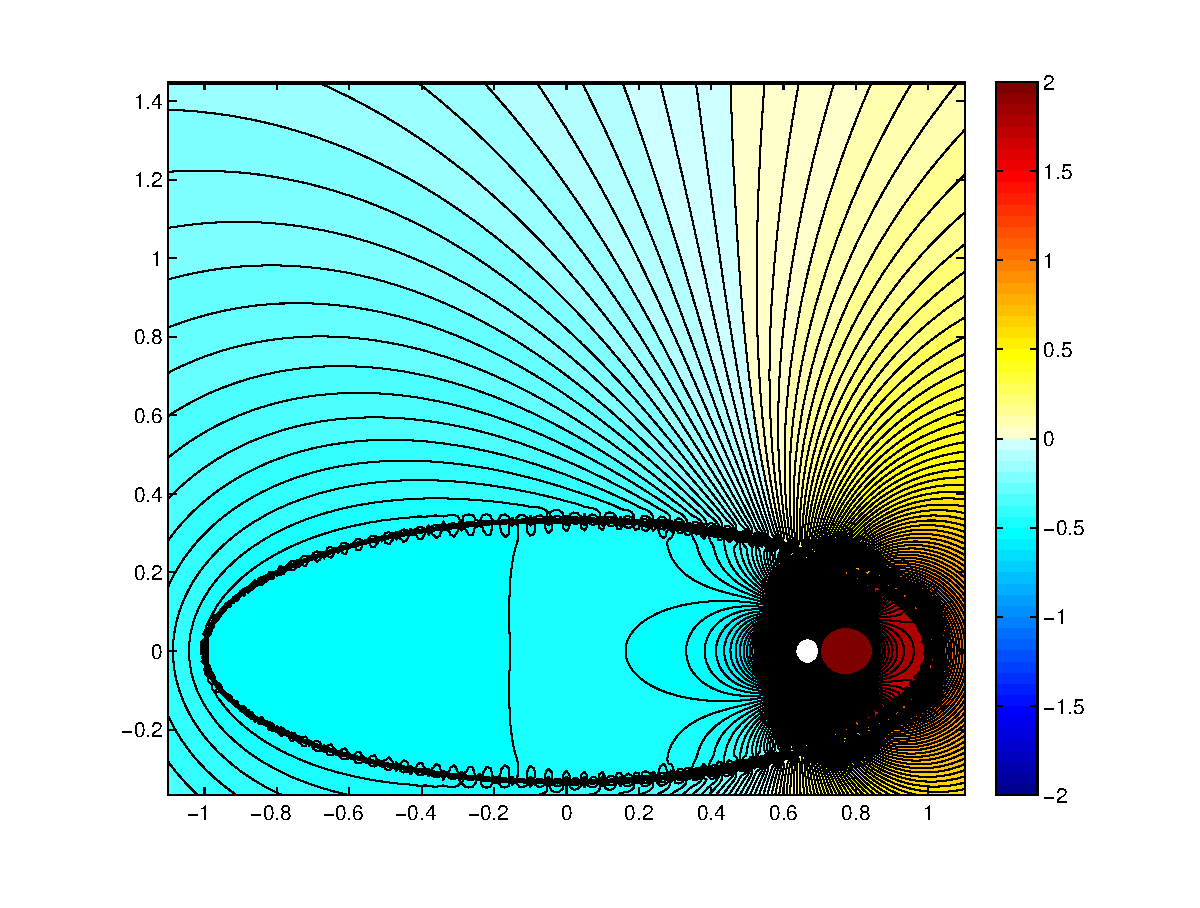
\includegraphics[width=0.45\textwidth]{model/fish_like_simul_without_anomaly.eps}}
\subfigure[Global overview, with the anomaly]{\label{fig:fish_like_simul}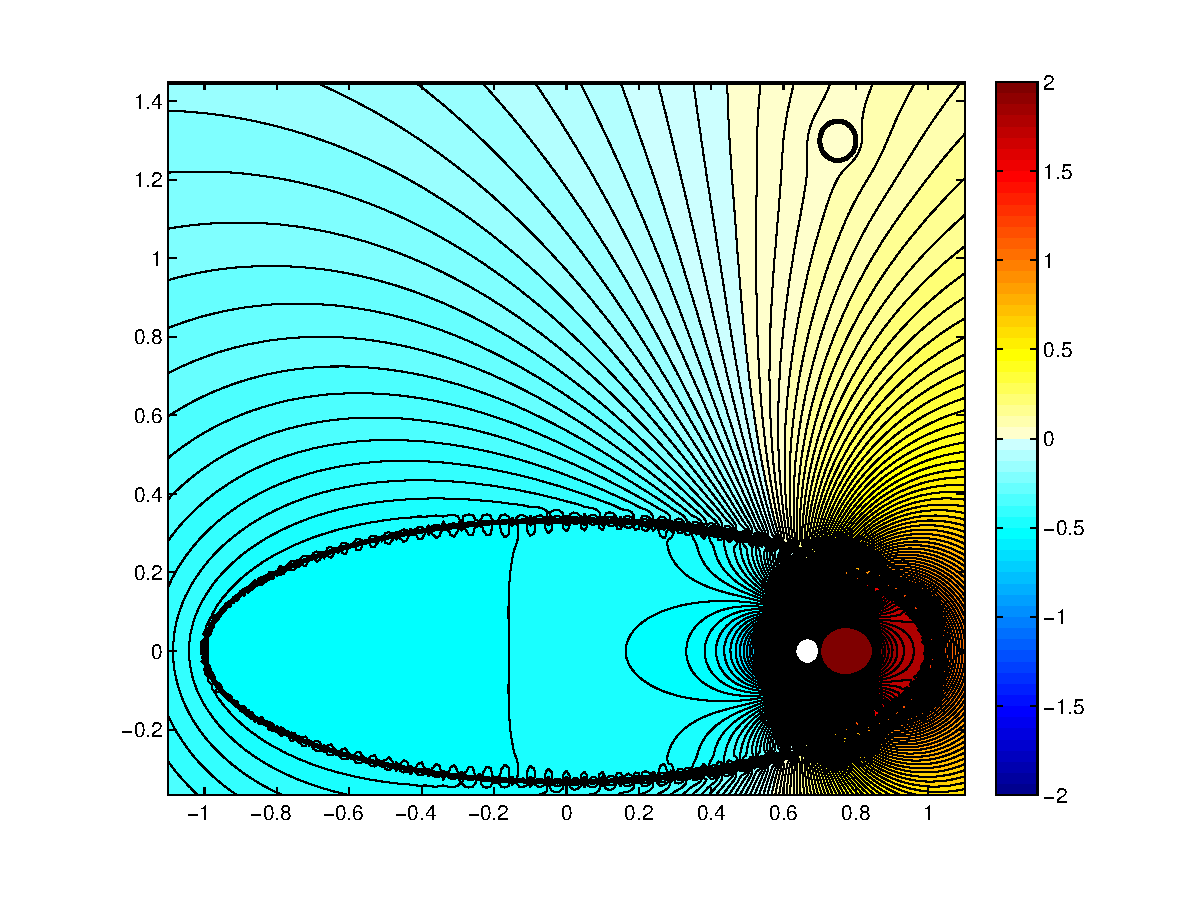
\includegraphics[width=0.45\textwidth]{model/fish_like_simul.eps}}
\subfigure[Zoom on the target]{\label{fig:zoom-target}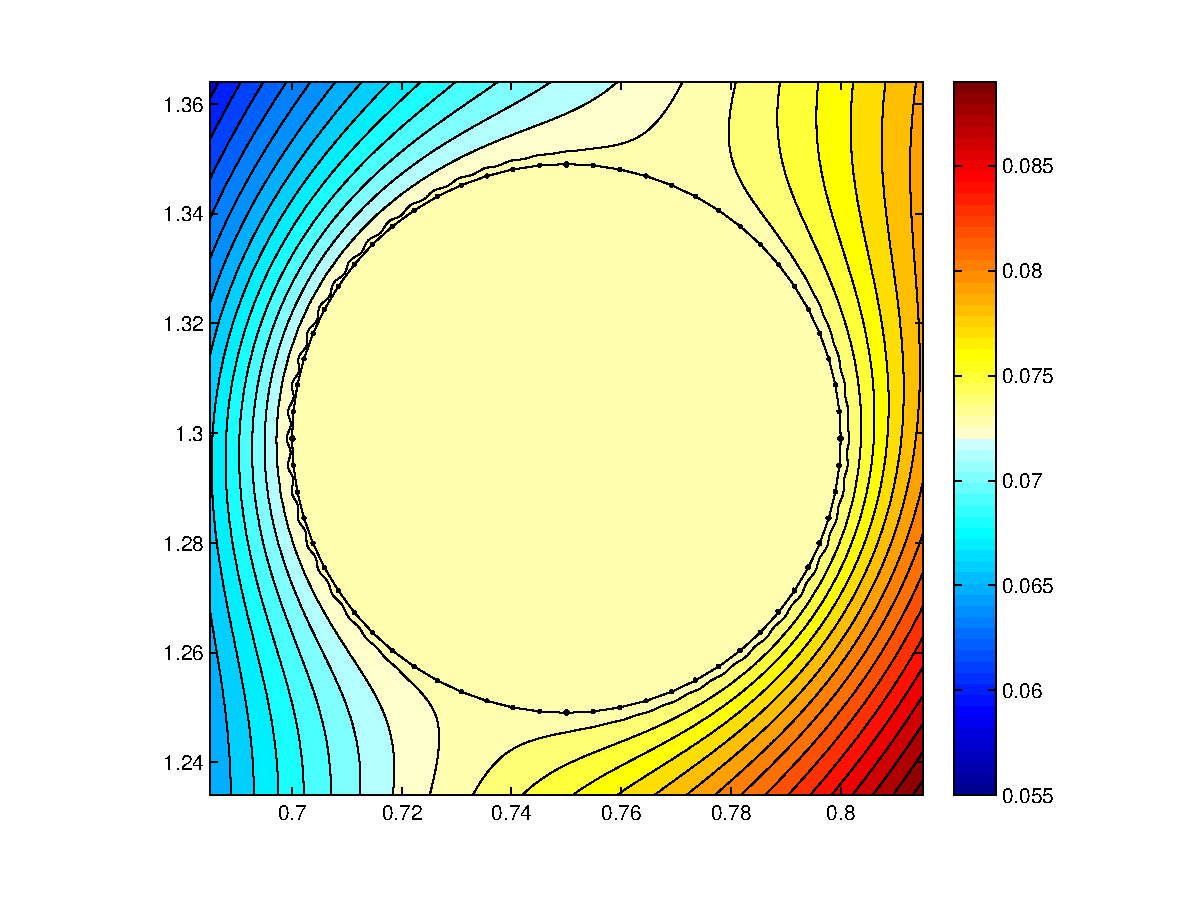
\includegraphics[width=0.45\textwidth]{model/zoom_anomaly.eps}}
\subfigure[Zoom on a target with different shape]{\label{fig:zoom-target-star}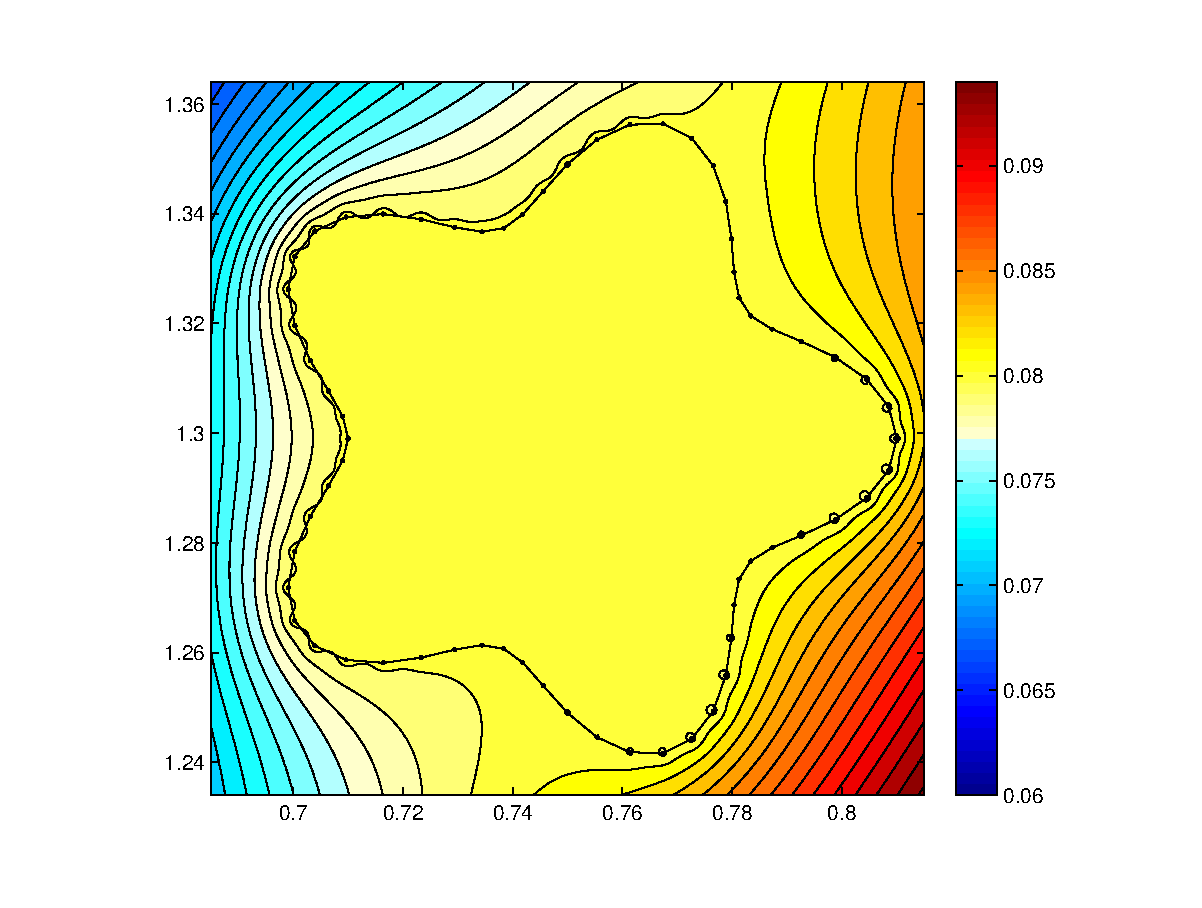
\includegraphics[width=0.45\textwidth]{model/zoom_anomaly_star.eps}}
\caption{Isopotentials for the cases described.}
\end{figure}

In Figure~\ref{fig:2disks}, we have placed two disks of conductivity $3$ and $5$,
at the points $(\cos(\pi/3),\sin(\pi/3))$ and $(0,\sin(\pi/3))$, respectively. The
electric field $u$ is plotted in Figure~\ref{fig:2disks_fwd}, the difference $u-U$
in Figure~\ref{fig:2disks_fwd_dipol}, and finally the field of the equivalent dipole
in Figure~\ref{fig:2disks_fwd_dipolEquiv}. This latter is given by the formula
shown in Proposition~\ref{propos2}.

\begin{figure}[!h]
\centering%
\subfigure[Electric potentiel $u$]{\label{fig:2disks_fwd}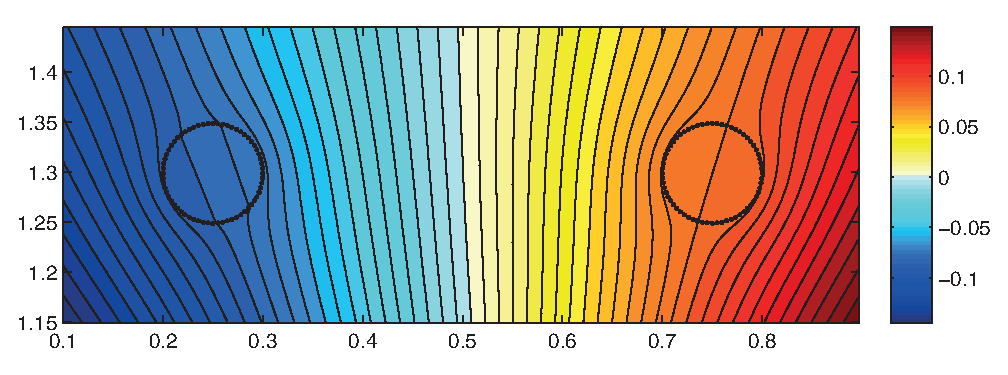
\includegraphics[width=\textwidth]{model/2disks_fwd.eps}}
\subfigure[Difference $u-U$]{\label{fig:2disks_fwd_dipol}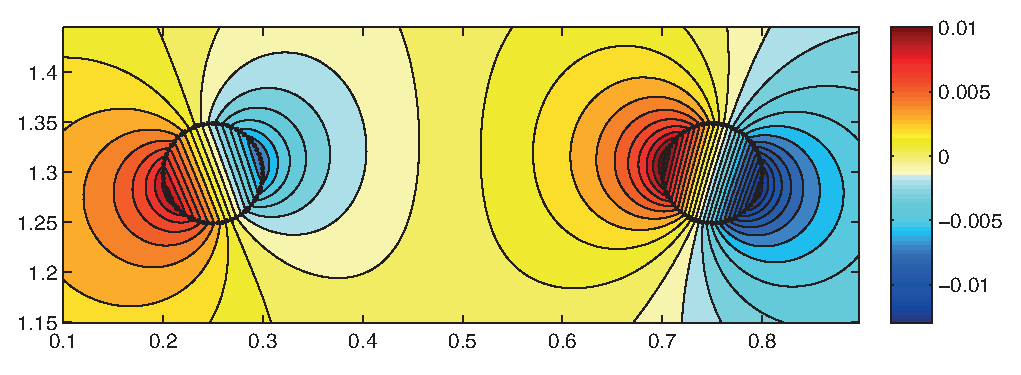
\includegraphics[width=\textwidth]{model/2disks_fwd_dipol.eps}}
\subfigure[Equivalent dipoles]{\label{fig:2disks_fwd_dipolEquiv}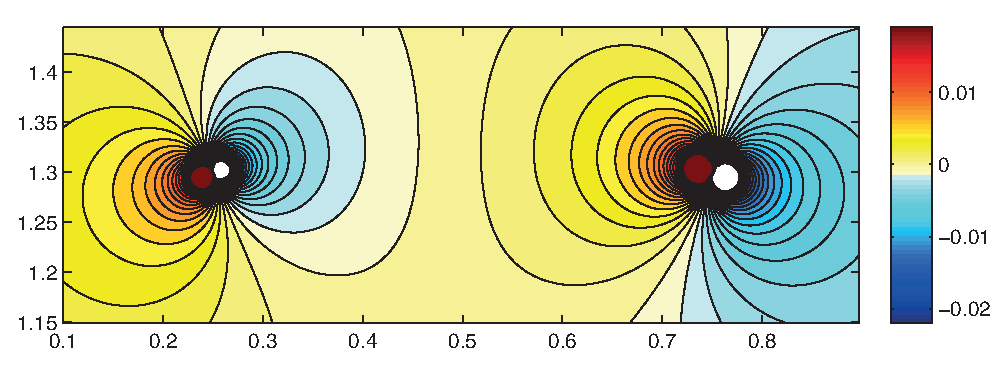
\includegraphics[width=\textwidth]{model/2disks_fwd_dipolEquiv.eps}}
\caption{Isopotentials for several objects.\label{fig:2disks}}
\end{figure}


\section{Conclusion}

In this chapter, we have proposed a complex conductivity model
for the electric field emitted by the fish. We have rigorously derived the boundary
conditions to be used, and the leading order terms of the transdermial currents
when an object is located in the vincinity of the fish. Finally, we have performed numerical simulations.

In the next chapter, we will use the approximation formulas derived 
in section~\ref{sec:perturbation-target} in order to localize the target.
